%File: anonymous-submission-latex-2026.tex
\documentclass[letterpaper]{article} % DO NOT CHANGE THIS
\usepackage[submission]{aaai2026}  % DO NOT CHANGE THIS
\usepackage{times}  % DO NOT CHANGE THIS
\usepackage{helvet}  % DO NOT CHANGE THIS
\usepackage{courier}  % DO NOT CHANGE THIS
\usepackage[hyphens]{url}  % DO NOT CHANGE THIS
\usepackage{graphicx} % DO NOT CHANGE THIS
\urlstyle{rm} % DO NOT CHANGE THIS
\def\UrlFont{\rm}  % DO NOT CHANGE THIS
\usepackage{natbib}  % DO NOT CHANGE THIS AND DO NOT ADD ANY OPTIONS TO IT
\usepackage{caption} % DO NOT CHANGE THIS AND DO NOT ADD ANY OPTIONS TO IT
\frenchspacing  % DO NOT CHANGE THIS
\setlength{\pdfpagewidth}{8.5in} % DO NOT CHANGE THIS
\setlength{\pdfpageheight}{11in} % DO NOT CHANGE THIS
%
% These are recommended to typeset algorithms but not required. See the subsubsection on algorithms. Remove them if you don't have algorithms in your paper.
% \usepackage{algorithm}
% \usepackage{algorithmic}
%%%%% NEW MATH DEFINITIONS %%%%%

\usepackage{amsmath}
\usepackage{amsfonts}
\usepackage{bm}

% Mark sections of captions for referring to divisions of figures
\newcommand{\figleft}{{\em (Left)}}
\newcommand{\figcenter}{{\em (Center)}}
\newcommand{\figright}{{\em (Right)}}
\newcommand{\figtop}{{\em (Top)}}
\newcommand{\figbottom}{{\em (Bottom)}}
\newcommand{\captiona}{{\em (a)}}
\newcommand{\captionb}{{\em (b)}}
\newcommand{\captionc}{{\em (c)}}
\newcommand{\captiond}{{\em (d)}}

% Highlight a newly defined term
\newcommand{\newterm}[1]{{\bf #1}}


% Figure reference, lower-case.
\def\figref#1{figure~\ref{#1}}
% Figure reference, capital. For start of sentence
\def\Figref#1{Figure~\ref{#1}}
\def\twofigref#1#2{figures \ref{#1} and \ref{#2}}
\def\quadfigref#1#2#3#4{figures \ref{#1}, \ref{#2}, \ref{#3} and \ref{#4}}
% Section reference, lower-case.
\def\secref#1{section~\ref{#1}}
% Section reference, capital.
\def\Secref#1{Section~\ref{#1}}
% Reference to two sections.
\def\twosecrefs#1#2{sections \ref{#1} and \ref{#2}}
% Reference to three sections.
\def\secrefs#1#2#3{sections \ref{#1}, \ref{#2} and \ref{#3}}
% Reference to an equation, lower-case.
\def\eqref#1{equation~\ref{#1}}
% Reference to an equation, upper case
\def\Eqref#1{Equation~\ref{#1}}
% A raw reference to an equation---avoid using if possible
\def\plaineqref#1{\ref{#1}}
% Reference to a chapter, lower-case.
\def\chapref#1{chapter~\ref{#1}}
% Reference to an equation, upper case.
\def\Chapref#1{Chapter~\ref{#1}}
% Reference to a range of chapters
\def\rangechapref#1#2{chapters\ref{#1}--\ref{#2}}
% Reference to an algorithm, lower-case.
\def\algref#1{algorithm~\ref{#1}}
% Reference to an algorithm, upper case.
\def\Algref#1{Algorithm~\ref{#1}}
\def\twoalgref#1#2{algorithms \ref{#1} and \ref{#2}}
\def\Twoalgref#1#2{Algorithms \ref{#1} and \ref{#2}}
% Reference to a part, lower case
\def\partref#1{part~\ref{#1}}
% Reference to a part, upper case
\def\Partref#1{Part~\ref{#1}}
\def\twopartref#1#2{parts \ref{#1} and \ref{#2}}

\def\ceil#1{\lceil #1 \rceil}
\def\floor#1{\lfloor #1 \rfloor}
\def\1{\bm{1}}
\newcommand{\train}{\mathcal{D}}
\newcommand{\valid}{\mathcal{D_{\mathrm{valid}}}}
\newcommand{\test}{\mathcal{D_{\mathrm{test}}}}

\def\eps{{\epsilon}}


% Random variables
\def\reta{{\textnormal{$\eta$}}}
\def\ra{{\textnormal{a}}}
\def\rb{{\textnormal{b}}}
\def\rc{{\textnormal{c}}}
\def\rd{{\textnormal{d}}}
\def\re{{\textnormal{e}}}
\def\rf{{\textnormal{f}}}
\def\rg{{\textnormal{g}}}
\def\rh{{\textnormal{h}}}
\def\ri{{\textnormal{i}}}
\def\rj{{\textnormal{j}}}
\def\rk{{\textnormal{k}}}
\def\rl{{\textnormal{l}}}
% rm is already a command, just don't name any random variables m
\def\rn{{\textnormal{n}}}
\def\ro{{\textnormal{o}}}
\def\rp{{\textnormal{p}}}
\def\rq{{\textnormal{q}}}
\def\rr{{\textnormal{r}}}
\def\rs{{\textnormal{s}}}
\def\rt{{\textnormal{t}}}
\def\ru{{\textnormal{u}}}
\def\rv{{\textnormal{v}}}
\def\rw{{\textnormal{w}}}
\def\rx{{\textnormal{x}}}
\def\ry{{\textnormal{y}}}
\def\rz{{\textnormal{z}}}

% Random vectors
\def\rvepsilon{{\mathbf{\epsilon}}}
\def\rvtheta{{\mathbf{\theta}}}
\def\rva{{\mathbf{a}}}
\def\rvb{{\mathbf{b}}}
\def\rvc{{\mathbf{c}}}
\def\rvd{{\mathbf{d}}}
\def\rve{{\mathbf{e}}}
\def\rvf{{\mathbf{f}}}
\def\rvg{{\mathbf{g}}}
\def\rvh{{\mathbf{h}}}
\def\rvu{{\mathbf{i}}}
\def\rvj{{\mathbf{j}}}
\def\rvk{{\mathbf{k}}}
\def\rvl{{\mathbf{l}}}
\def\rvm{{\mathbf{m}}}
\def\rvn{{\mathbf{n}}}
\def\rvo{{\mathbf{o}}}
\def\rvp{{\mathbf{p}}}
\def\rvq{{\mathbf{q}}}
\def\rvr{{\mathbf{r}}}
\def\rvs{{\mathbf{s}}}
\def\rvt{{\mathbf{t}}}
\def\rvu{{\mathbf{u}}}
\def\rvv{{\mathbf{v}}}
\def\rvw{{\mathbf{w}}}
\def\rvx{{\mathbf{x}}}
\def\rvy{{\mathbf{y}}}
\def\rvz{{\mathbf{z}}}

% Elements of random vectors
\def\erva{{\textnormal{a}}}
\def\ervb{{\textnormal{b}}}
\def\ervc{{\textnormal{c}}}
\def\ervd{{\textnormal{d}}}
\def\erve{{\textnormal{e}}}
\def\ervf{{\textnormal{f}}}
\def\ervg{{\textnormal{g}}}
\def\ervh{{\textnormal{h}}}
\def\ervi{{\textnormal{i}}}
\def\ervj{{\textnormal{j}}}
\def\ervk{{\textnormal{k}}}
\def\ervl{{\textnormal{l}}}
\def\ervm{{\textnormal{m}}}
\def\ervn{{\textnormal{n}}}
\def\ervo{{\textnormal{o}}}
\def\ervp{{\textnormal{p}}}
\def\ervq{{\textnormal{q}}}
\def\ervr{{\textnormal{r}}}
\def\ervs{{\textnormal{s}}}
\def\ervt{{\textnormal{t}}}
\def\ervu{{\textnormal{u}}}
\def\ervv{{\textnormal{v}}}
\def\ervw{{\textnormal{w}}}
\def\ervx{{\textnormal{x}}}
\def\ervy{{\textnormal{y}}}
\def\ervz{{\textnormal{z}}}

% Random matrices
\def\rmA{{\mathbf{A}}}
\def\rmB{{\mathbf{B}}}
\def\rmC{{\mathbf{C}}}
\def\rmD{{\mathbf{D}}}
\def\rmE{{\mathbf{E}}}
\def\rmF{{\mathbf{F}}}
\def\rmG{{\mathbf{G}}}
\def\rmH{{\mathbf{H}}}
\def\rmI{{\mathbf{I}}}
\def\rmJ{{\mathbf{J}}}
\def\rmK{{\mathbf{K}}}
\def\rmL{{\mathbf{L}}}
\def\rmM{{\mathbf{M}}}
\def\rmN{{\mathbf{N}}}
\def\rmO{{\mathbf{O}}}
\def\rmP{{\mathbf{P}}}
\def\rmQ{{\mathbf{Q}}}
\def\rmR{{\mathbf{R}}}
\def\rmS{{\mathbf{S}}}
\def\rmT{{\mathbf{T}}}
\def\rmU{{\mathbf{U}}}
\def\rmV{{\mathbf{V}}}
\def\rmW{{\mathbf{W}}}
\def\rmX{{\mathbf{X}}}
\def\rmY{{\mathbf{Y}}}
\def\rmZ{{\mathbf{Z}}}

% Elements of random matrices
\def\ermA{{\textnormal{A}}}
\def\ermB{{\textnormal{B}}}
\def\ermC{{\textnormal{C}}}
\def\ermD{{\textnormal{D}}}
\def\ermE{{\textnormal{E}}}
\def\ermF{{\textnormal{F}}}
\def\ermG{{\textnormal{G}}}
\def\ermH{{\textnormal{H}}}
\def\ermI{{\textnormal{I}}}
\def\ermJ{{\textnormal{J}}}
\def\ermK{{\textnormal{K}}}
\def\ermL{{\textnormal{L}}}
\def\ermM{{\textnormal{M}}}
\def\ermN{{\textnormal{N}}}
\def\ermO{{\textnormal{O}}}
\def\ermP{{\textnormal{P}}}
\def\ermQ{{\textnormal{Q}}}
\def\ermR{{\textnormal{R}}}
\def\ermS{{\textnormal{S}}}
\def\ermT{{\textnormal{T}}}
\def\ermU{{\textnormal{U}}}
\def\ermV{{\textnormal{V}}}
\def\ermW{{\textnormal{W}}}
\def\ermX{{\textnormal{X}}}
\def\ermY{{\textnormal{Y}}}
\def\ermZ{{\textnormal{Z}}}

% Vectors
\def\vzero{{\bm{0}}}
\def\vone{{\bm{1}}}
\def\vmu{{\bm{\mu}}}
\def\vtheta{{\bm{\theta}}}
\def\va{{\bm{a}}}
\def\vb{{\bm{b}}}
\def\vc{{\bm{c}}}
\def\vd{{\bm{d}}}
\def\ve{{\bm{e}}}
\def\vf{{\bm{f}}}
\def\vg{{\bm{g}}}
\def\vh{{\bm{h}}}
\def\vi{{\bm{i}}}
\def\vj{{\bm{j}}}
\def\vk{{\bm{k}}}
\def\vl{{\bm{l}}}
\def\vm{{\bm{m}}}
\def\vn{{\bm{n}}}
\def\vo{{\bm{o}}}
\def\vp{{\bm{p}}}
\def\vq{{\bm{q}}}
\def\vr{{\bm{r}}}
\def\vs{{\bm{s}}}
\def\vt{{\bm{t}}}
\def\vu{{\bm{u}}}
\def\vv{{\bm{v}}}
\def\vw{{\bm{w}}}
\def\vx{{\bm{x}}}
\def\vy{{\bm{y}}}
\def\vz{{\bm{z}}}

% Elements of vectors
\def\evalpha{{\alpha}}
\def\evbeta{{\beta}}
\def\evepsilon{{\epsilon}}
\def\evlambda{{\lambda}}
\def\evomega{{\omega}}
\def\evmu{{\mu}}
\def\evpsi{{\psi}}
\def\evsigma{{\sigma}}
\def\evtheta{{\theta}}
\def\eva{{a}}
\def\evb{{b}}
\def\evc{{c}}
\def\evd{{d}}
\def\eve{{e}}
\def\evf{{f}}
\def\evg{{g}}
\def\evh{{h}}
\def\evi{{i}}
\def\evj{{j}}
\def\evk{{k}}
\def\evl{{l}}
\def\evm{{m}}
\def\evn{{n}}
\def\evo{{o}}
\def\evp{{p}}
\def\evq{{q}}
\def\evr{{r}}
\def\evs{{s}}
\def\evt{{t}}
\def\evu{{u}}
\def\evv{{v}}
\def\evw{{w}}
\def\evx{{x}}
\def\evy{{y}}
\def\evz{{z}}

% Matrix
\def\mA{{\bm{A}}}
\def\mB{{\bm{B}}}
\def\mC{{\bm{C}}}
\def\mD{{\bm{D}}}
\def\mE{{\bm{E}}}
\def\mF{{\bm{F}}}
\def\mG{{\bm{G}}}
\def\mH{{\bm{H}}}
\def\mI{{\bm{I}}}
\def\mJ{{\bm{J}}}
\def\mK{{\bm{K}}}
\def\mL{{\bm{L}}}
\def\mM{{\bm{M}}}
\def\mN{{\bm{N}}}
\def\mO{{\bm{O}}}
\def\mP{{\bm{P}}}
\def\mQ{{\bm{Q}}}
\def\mR{{\bm{R}}}
\def\mS{{\bm{S}}}
\def\mT{{\bm{T}}}
\def\mU{{\bm{U}}}
\def\mV{{\bm{V}}}
\def\mW{{\bm{W}}}
\def\mX{{\bm{X}}}
\def\mY{{\bm{Y}}}
\def\mZ{{\bm{Z}}}
\def\mBeta{{\bm{\beta}}}
\def\mPhi{{\bm{\Phi}}}
\def\mLambda{{\bm{\Lambda}}}
\def\mSigma{{\bm{\Sigma}}}

% Tensor
\DeclareMathAlphabet{\mathsfit}{\encodingdefault}{\sfdefault}{m}{sl}
\SetMathAlphabet{\mathsfit}{bold}{\encodingdefault}{\sfdefault}{bx}{n}
\newcommand{\tens}[1]{\bm{\mathsfit{#1}}}
\def\tA{{\tens{A}}}
\def\tB{{\tens{B}}}
\def\tC{{\tens{C}}}
\def\tD{{\tens{D}}}
\def\tE{{\tens{E}}}
\def\tF{{\tens{F}}}
\def\tG{{\tens{G}}}
\def\tH{{\tens{H}}}
\def\tI{{\tens{I}}}
\def\tJ{{\tens{J}}}
\def\tK{{\tens{K}}}
\def\tL{{\tens{L}}}
\def\tM{{\tens{M}}}
\def\tN{{\tens{N}}}
\def\tO{{\tens{O}}}
\def\tP{{\tens{P}}}
\def\tQ{{\tens{Q}}}
\def\tR{{\tens{R}}}
\def\tS{{\tens{S}}}
\def\tT{{\tens{T}}}
\def\tU{{\tens{U}}}
\def\tV{{\tens{V}}}
\def\tW{{\tens{W}}}
\def\tX{{\tens{X}}}
\def\tY{{\tens{Y}}}
\def\tZ{{\tens{Z}}}


% Graph
\def\gA{{\mathcal{A}}}
\def\gB{{\mathcal{B}}}
\def\gC{{\mathcal{C}}}
\def\gD{{\mathcal{D}}}
\def\gE{{\mathcal{E}}}
\def\gF{{\mathcal{F}}}
\def\gG{{\mathcal{G}}}
\def\gH{{\mathcal{H}}}
\def\gI{{\mathcal{I}}}
\def\gJ{{\mathcal{J}}}
\def\gK{{\mathcal{K}}}
\def\gL{{\mathcal{L}}}
\def\gM{{\mathcal{M}}}
\def\gN{{\mathcal{N}}}
\def\gO{{\mathcal{O}}}
\def\gP{{\mathcal{P}}}
\def\gQ{{\mathcal{Q}}}
\def\gR{{\mathcal{R}}}
\def\gS{{\mathcal{S}}}
\def\gT{{\mathcal{T}}}
\def\gU{{\mathcal{U}}}
\def\gV{{\mathcal{V}}}
\def\gW{{\mathcal{W}}}
\def\gX{{\mathcal{X}}}
\def\gY{{\mathcal{Y}}}
\def\gZ{{\mathcal{Z}}}

% Sets
\def\sA{{\mathbb{A}}}
\def\sB{{\mathbb{B}}}
\def\sC{{\mathbb{C}}}
\def\sD{{\mathbb{D}}}
% Don't use a set called E, because this would be the same as our symbol
% for expectation.
\def\sF{{\mathbb{F}}}
\def\sG{{\mathbb{G}}}
\def\sH{{\mathbb{H}}}
\def\sI{{\mathbb{I}}}
\def\sJ{{\mathbb{J}}}
\def\sK{{\mathbb{K}}}
\def\sL{{\mathbb{L}}}
\def\sM{{\mathbb{M}}}
\def\sN{{\mathbb{N}}}
\def\sO{{\mathbb{O}}}
\def\sP{{\mathbb{P}}}
\def\sQ{{\mathbb{Q}}}
\def\sR{{\mathbb{R}}}
\def\sS{{\mathbb{S}}}
\def\sT{{\mathbb{T}}}
\def\sU{{\mathbb{U}}}
\def\sV{{\mathbb{V}}}
\def\sW{{\mathbb{W}}}
\def\sX{{\mathbb{X}}}
\def\sY{{\mathbb{Y}}}
\def\sZ{{\mathbb{Z}}}

% Entries of a matrix
\def\emLambda{{\Lambda}}
\def\emA{{A}}
\def\emB{{B}}
\def\emC{{C}}
\def\emD{{D}}
\def\emE{{E}}
\def\emF{{F}}
\def\emG{{G}}
\def\emH{{H}}
\def\emI{{I}}
\def\emJ{{J}}
\def\emK{{K}}
\def\emL{{L}}
\def\emM{{M}}
\def\emN{{N}}
\def\emO{{O}}
\def\emP{{P}}
\def\emQ{{Q}}
\def\emR{{R}}
\def\emS{{S}}
\def\emT{{T}}
\def\emU{{U}}
\def\emV{{V}}
\def\emW{{W}}
\def\emX{{X}}
\def\emY{{Y}}
\def\emZ{{Z}}
\def\emSigma{{\Sigma}}

% entries of a tensor
% Same font as tensor, without \bm wrapper
\newcommand{\etens}[1]{\mathsfit{#1}}
\def\etLambda{{\etens{\Lambda}}}
\def\etA{{\etens{A}}}
\def\etB{{\etens{B}}}
\def\etC{{\etens{C}}}
\def\etD{{\etens{D}}}
\def\etE{{\etens{E}}}
\def\etF{{\etens{F}}}
\def\etG{{\etens{G}}}
\def\etH{{\etens{H}}}
\def\etI{{\etens{I}}}
\def\etJ{{\etens{J}}}
\def\etK{{\etens{K}}}
\def\etL{{\etens{L}}}
\def\etM{{\etens{M}}}
\def\etN{{\etens{N}}}
\def\etO{{\etens{O}}}
\def\etP{{\etens{P}}}
\def\etQ{{\etens{Q}}}
\def\etR{{\etens{R}}}
\def\etS{{\etens{S}}}
\def\etT{{\etens{T}}}
\def\etU{{\etens{U}}}
\def\etV{{\etens{V}}}
\def\etW{{\etens{W}}}
\def\etX{{\etens{X}}}
\def\etY{{\etens{Y}}}
\def\etZ{{\etens{Z}}}

% The true underlying data generating distribution
\newcommand{\pdata}{p_{\rm{data}}}
% The empirical distribution defined by the training set
\newcommand{\ptrain}{\hat{p}_{\rm{data}}}
\newcommand{\Ptrain}{\hat{P}_{\rm{data}}}
% The model distribution
\newcommand{\pmodel}{p_{\rm{model}}}
\newcommand{\Pmodel}{P_{\rm{model}}}
\newcommand{\ptildemodel}{\tilde{p}_{\rm{model}}}
% Stochastic autoencoder distributions
\newcommand{\pencode}{p_{\rm{encoder}}}
\newcommand{\pdecode}{p_{\rm{decoder}}}
\newcommand{\precons}{p_{\rm{reconstruct}}}

\newcommand{\laplace}{\mathrm{Laplace}} % Laplace distribution

\newcommand{\E}{\mathbb{E}}
\newcommand{\Ls}{\mathcal{L}}
\newcommand{\R}{\mathbb{R}}
\newcommand{\emp}{\tilde{p}}
\newcommand{\lr}{\alpha}
\newcommand{\reg}{\lambda}
\newcommand{\rect}{\mathrm{rectifier}}
\newcommand{\softmax}{\mathrm{softmax}}
\newcommand{\sigmoid}{\sigma}
\newcommand{\softplus}{\zeta}
\newcommand{\KL}{D_{\mathrm{KL}}}
\newcommand{\Var}{\mathrm{Var}}
\newcommand{\standarderror}{\mathrm{SE}}
\newcommand{\Cov}{\mathrm{Cov}}
% Wolfram Mathworld says $L^2$ is for function spaces and $\ell^2$ is for vectors
% But then they seem to use $L^2$ for vectors throughout the site, and so does
% wikipedia.
\newcommand{\normlzero}{L^0}
\newcommand{\normlone}{L^1}
\newcommand{\normltwo}{L^2}
\newcommand{\normlp}{L^p}
\newcommand{\normmax}{L^\infty}

\newcommand{\parents}{Pa} % See usage in notation.tex. Chosen to match Daphne's book.

\DeclareMathOperator*{\argmax}{arg\,max}
\DeclareMathOperator*{\argmin}{arg\,min}

\DeclareMathOperator{\sign}{sign}
\DeclareMathOperator{\Tr}{Tr}
\let\ab\allowbreak

%
% These are are recommended to typeset listings but not required. See the subsubsection on listing. Remove this block if you don't have listings in your paper.
\usepackage{newfloat}
\usepackage{listings}

% ready for submission
% \usepackage{iclr2025_conference}
% \usepackage{hyperref}
% \usepackage{url}
\usepackage{graphicx}
\usepackage{graphicx}
\usepackage{subfigure}
\usepackage{booktabs} % for professional tables
% For theorems and such
\usepackage{amsmath}
\usepackage{amssymb}
\usepackage{mathtools}
\usepackage{amsthm}
\usepackage{placeins}
\theoremstyle{plain}
\newtheorem{theorem}{Theorem}[section]
\newtheorem{proposition}[theorem]{Proposition}
\newtheorem{lemma}[theorem]{Lemma}
\newtheorem{corollary}[theorem]{Corollary}
\theoremstyle{definition}
\newtheorem{definition}[theorem]{Definition}
\newtheorem{assumption}[theorem]{Assumption}
\theoremstyle{remark}
\newtheorem{remark}[theorem]{Remark}

\usepackage{xcolor}
\usepackage{colortbl}
\usepackage{algorithm}
\usepackage{algpseudocode}
\usepackage{rotating}
\usepackage{caption}

\usepackage{afterpage}

\newcommand\blankpage{%
    \null
    \thispagestyle{empty}%
    \addtocounter{page}{-1}%
    \newpage}
% to compile a preprint version, e.g., for submission to arXiv, add add the
% [preprint] option:
%     \usepackage[preprint]{neurips_2025}


% to compile a camera-ready version, add the [final] option, e.g.:
%     \usepackage[final]{neurips_2025}


% to avoid loading the natbib package, add option nonatbib:
%    \usepackage[nonatbib]{neurips_2025}


\usepackage[utf8]{inputenc} % allow utf-8 input
\usepackage[T1]{fontenc}    % use 8-bit T1 fonts
% \usepackage{hyperref}       % hyperlinks
\usepackage{url}            % simple URL typesetting
\usepackage{booktabs}       % professional-quality tables
\usepackage{amsfonts}       % blackboard math symbols
\usepackage{nicefrac}       % compact symbols for 1/2, etc.
\usepackage{microtype}      % microtypography
\usepackage{xcolor}         % colors

\DeclareCaptionStyle{ruled}{labelfont=normalfont,labelsep=colon,strut=off} % DO NOT CHANGE THIS
\lstset{%
	basicstyle={\footnotesize\ttfamily},% footnotesize acceptable for monospace
	numbers=left,numberstyle=\footnotesize,xleftmargin=2em,% show line numbers, remove this entire line if you don't want the numbers.
	aboveskip=0pt,belowskip=0pt,%
	showstringspaces=false,tabsize=2,breaklines=true}
\floatstyle{ruled}
\newfloat{listing}{tb}{lst}{}
\floatname{listing}{Listing}
%
% Keep the \pdfinfo as shown here. There's no need
% for you to add the /Title and /Author tags.
\pdfinfo{
/TemplateVersion (2026.1)
}

% DISALLOWED PACKAGES
% \usepackage{authblk} -- This package is specifically forbidden
% \usepackage{balance} -- This package is specifically forbidden
% \usepackage{color (if used in text)
% \usepackage{CJK} -- This package is specifically forbidden
% \usepackage{float} -- This package is specifically forbidden
% \usepackage{flushend} -- This package is specifically forbidden
% \usepackage{fontenc} -- This package is specifically forbidden
% \usepackage{fullpage} -- This package is specifically forbidden
% \usepackage{geometry} -- This package is specifically forbidden
% \usepackage{grffile} -- This package is specifically forbidden
% \usepackage{hyperref} -- This package is specifically forbidden
% \usepackage{navigator} -- This package is specifically forbidden
% (or any other package that embeds links such as navigator or hyperref)
% \indentfirst} -- This package is specifically forbidden
% \layout} -- This package is specifically forbidden
% \multicol} -- This package is specifically forbidden
% \nameref} -- This package is specifically forbidden
% \usepackage{savetrees} -- This package is specifically forbidden
% \usepackage{setspace} -- This package is specifically forbidden
% \usepackage{stfloats} -- This package is specifically forbidden
% \usepackage{tabu} -- This package is specifically forbidden
% \usepackage{titlesec} -- This package is specifically forbidden
% \usepackage{tocbibind} -- This package is specifically forbidden
% \usepackage{ulem} -- This package is specifically forbidden
% \usepackage{wrapfig} -- This package is specifically forbidden
% DISALLOWED COMMANDS
% \nocopyright -- Your paper will not be published if you use this command
% \addtolength -- This command may not be used
% \balance -- This command may not be used
% \baselinestretch -- Your paper will not be published if you use this command
% \clearpage -- No page breaks of any kind may be used for the final version of your paper
% \columnsep -- This command may not be used
% \newpage -- No page breaks of any kind may be used for the final version of your paper
% \pagebreak -- No page breaks of any kind may be used for the final version of your paperr
% \pagestyle -- This command may not be used
% \tiny -- This is not an acceptable font size.
% \vspace{- -- No negative value may be used in proximity of a caption, figure, table, section, subsection, subsubsection, or reference
% \vskip{- -- No negative value may be used to alter spacing above or below a caption, figure, table, section, subsection, subsubsection, or reference

\setcounter{secnumdepth}{2} %May be changed to 1 or 2 if section numbers are desired.

% The file aaai2026.sty is the style file for AAAI Press
% proceedings, working notes, and technical reports.
%

% Title

% Your title must be in mixed case, not sentence case.
% That means all verbs (including short verbs like be, is, using,and go),
% nouns, adverbs, adjectives should be capitalized, including both words in hyphenated terms, while
% articles, conjunctions, and prepositions are lower case unless they
% directly follow a colon or long dash
\title{Domain Feature Collapse: Implications for Out-of-Distribution Detection and Solutions}
\author{
    %Authors
    % All authors must be in the same font size and format.
    Written by AAAI Press Staff\textsuperscript{\rm 1}\thanks{With help from the AAAI Publications Committee.}\\
    AAAI Style Contributions by Pater Patel Schneider,
    Sunil Issar,\\
    J. Scott Penberthy,
    George Ferguson,
    Hans Guesgen,
    Francisco Cruz\equalcontrib,
    Marc Pujol-Gonzalez\equalcontrib
}
\affiliations{
    %Afiliations
    \textsuperscript{\rm 1}Association for the Advancement of Artificial Intelligence\\
    % If you have multiple authors and multiple affiliations
    % use superscripts in text and roman font to identify them.
    % For example,

    % Sunil Issar\textsuperscript{\rm 2},
    % J. Scott Penberthy\textsuperscript{\rm 3},
    % George Ferguson\textsuperscript{\rm 4},
    % Hans Guesgen\textsuperscript{\rm 5}
    % Note that the comma should be placed after the superscript

    1101 Pennsylvania Ave, NW Suite 300\\
    Washington, DC 20004 USA\\
    % email address must be in roman text type, not monospace or sans serif
    proceedings-questions@aaai.org
%
% See more examples next
}

%Example, Single Author, ->> remove \iffalse,\fi and place them surrounding AAAI title to use it
\iffalse
\title{Domain Feature Collapse: Implications for Out-of-Distribution Detection and Solutions}
\author {
    Author Name
}
\affiliations{
    Affiliation\\
    Affiliation Line 2\\
    name@example.com
}
\fi

\iffalse
%Example, Multiple Authors, ->> remove \iffalse,\fi and place them surrounding AAAI title to use it
\title{My Publication Title --- Multiple Authors}
\author {
    % Authors
    First Author Name\textsuperscript{\rm 1},
    Second Author Name\textsuperscript{\rm 2},
    Third Author Name\textsuperscript{\rm 1}
}
\affiliations {
    % Affiliations
    \textsuperscript{\rm 1}Affiliation 1\\
    \textsuperscript{\rm 2}Affiliation 2\\
    firstAuthor@affiliation1.com, secondAuthor@affilation2.com, thirdAuthor@affiliation1.com
}
\fi


% REMOVE THIS: bibentry
% This is only needed to show inline citations in the guidelines document. You should not need it and can safely delete it.
\usepackage{bibentry}
% END REMOVE bibentry

\begin{document}

\maketitle

\begin{abstract}

The deployment of deep neural networks in safety-critical domains necessitates robust out-of-distribution (OOD) detection. While existing methods demonstrate strong performance on diverse multi-domain benchmarks, they are not specifically tailored to real-world applications where in-distribution data often originates from a single, narrow domain. This paper identifies and theoretically proves the existence of a critical issue that is unique to single-domain settings: \emph{domain feature collapse}. We show, through information theory and bottleneck compression, that models trained on a single domain dataset with a class label objective learn representations that discard domain-specific features, relying predominantly on class features. This collapse results in significantly higher error rates for out-of-domain OOD detection, a failure mode not adequately captured by traditional multi-domain benchmarks. To combat this, we introduce a two-stage domain filtering process as a simple and effective solution. Domain filtering leverages an initial stage to determine if an input is in-domain before subsequently applying a standard OOD detector. Additionally, we propose the Domain Bench, a new benchmark comprised of various single-domain datasets, providing empirical evidence for domain feature collapse as well as a testbed for evaluating solutions. Our experimental results validate our theoretical findings, showing that existing methods struggle with out-of-domain detection in single-domain contexts and that incorporating domain filtering substantially improves performance in these scenarios, underscoring its importance for reliable OOD detection in single-domain applications.

\end{abstract}

\section{Introduction}
\label{sec:intro}

The deployment of deep neural networks (DNNs) in safety-critical domains -- such as autonomous driving \citep{ramanagopal2018failing}, biometric authentication \citep{wang2021deep}, and medical diagnostics \citep{bakator2018deep} -- has spurred growing interest in ensuring their reliability. In these contexts, the traditional closed-world assumption \citep{krizhevsky2012imagenet}, where training and test data are drawn i.i.d. from the same in-distribution (ID), is no longer valid. Instead, models must operate under open-world conditions \citep{drummond2006open}, where inputs encountered at test time may stem from entirely different, out-of-distribution (OOD) sources. This reality necessitates robust OOD detection methods, which aim to flag inputs whose labels were not seen during training. The rationale is straightforward: we must prevent high-stakes systems from acting on predictions that are inherently invalid due to unseen or unfamiliar inputs.

Many state-of-the-art OOD detection methods demonstrate strong performance across established benchmarks \citep{zhang2023openood}. However, these benchmarks almost exclusively use in-distribution sets that contain samples and classes from a wide variety of domains, such as \citep{zhang2023openood}, which explicitly emphasize performance on CIFAR10/100 \citep{cifar10} and ImageNet \citep{deng2009imagenet}. While this approach provides a broad testbed for evaluating OOD robustness, it implicitly biases models and methods toward handling multi-domain in-distribution settings. As a result, there exists a gap in the literature: current OOD detection techniques are largely tailored to scenarios where the ID data is inherently diverse, rather than narrow or homogeneous. This raises concern as to how well these methods generalize to real-world applications where ID data may come from a single domain or task-specific distribution.

The single domain setting is understudied in bleeding edge OOD detection research, yet it has been heavily studied in the application of OOD methods for downstream tasks. Single-domain OOD detection is particularly important in application areas such as medical imaging \citep{zhang2021out}, satellite imagery \citep{ekim2024distribution}, and agriculture \citep{saadati2024out}, where models are often deployed in narrowly scoped environments with highly consistent data characteristics. This creates a domain mismatch between the theoretical efforts of the best OOD detection researchers and the practitioners who would benefit greatly from their research. 

Surprisingly, there is a fatal flaw in OOD detection that only occurs in single domain settings. This paper introduces the concept of and theoretically proves the existence of \textbf{domain feature collapse}. Through information theory and bottleneck compression, we show that artificial neural networks will remove domain specific features from their learned representations, under the single domain setting. This leads to a situation where OOD detection relies solely on class-specific features, while ignoring domain-specific features (e.g., knowing that an image is an X-ray does not help in detecting the disease depicted by the X-ray, but would help in OOD detection). Unfortunately, this failure results in higher OOD detection error rates when the ID set is single domain versus multi-domain. Since this mode of OOD detection failure rarely occurs for multi-domain ID sets, it is difficult to identify in the commonly used OOD benchmarks. 

To address the issue of domain feature collapse, we introduce a new benchmark to evaluate the performance of OOD detection algorithms in the single domain setting. This benchmark covers data from a wide variety of singular domains, including medical imaging, agriculture, satellite imagery, and more. We also propose a simple but effective solution to domain feature collapse, a two stage domain filtering process. Our theory suggests that it is absolutely necessary to address the issue of domain feature collapse in order to ensure safe OOD detection in single domain settings. 

Our key contributions are as follows:
\begin{itemize}
\item \textbf{Domain Feature Collapse}: Through bottleneck compression, we prove that training on a single domain results in a learned representation that contains no discriminative information regarding that particular domain, as this domain would be independent of the class within the context of the training dataset. We label this behavior as domain feature collapse, where a class label-supervised model will only learn class features and ignore domain features. 

\item \textbf{Domain Filtering}: We introduce a simple and consistent solution to the problem of domain feature collapse that allows any existing OOD detection algorithm to maintain high performance for both in-domain and out-of-domain OOD detection.  

\item \textbf{Domain Bench}: We introduce multiple single-domain datasets to provide empirical evidence of domain feature collapse across a wide variety of domains. We release source code to run these benchmarks following the OpenOOD framework \citep{zhang2023openood} in order to improve future research in single domain settings \footnote{see supplementary material for anonymized repository}.

%\footnote{https://anonymous.4open.science/r/DFC-6C35/README.md}


\end{itemize}


\section{Preliminaries}
\label{sec:preliminaries}

\subsection{Out-of-Distribution Detection}
\label{sec:ood_detection}

The task of out-of-distribution detection is to identify a semantic shift in the data \citep{yang2021generalized}. This is determining when no predicted label could match the true label $\rvy \notin \sY_{in}$, where $\sY_{in}$ represents the set of in-distribution training labels. In this case, we would consider the semantic space of the sample and the training distribution to be different; this represents a semantic shift. We can then express the probability that a sample is out-of-distribution as $P(\rvy \notin \sY_{in} | \rvx)$. \textcolor{black}{One baseline method to calculate $P(\rvy \notin \sY_{in} | \rvx)$ is to take $1 - \texttt{MSP}(\rvx)$, where $\texttt{MSP}$ is the maximum softmax probability extracted from a classifier for a particular datapoint.}

Furthermore, we are only concerned with labels that can be generated using only $\rvx$, via function $f$ which depends solely on $\rvx$ and no other information. Note that $f_\rvy$ may represent human labelers that generate $\rvy$. If we consider $\sY_{all}$ as the set of all possible labels that can be generated from $f_\rvy(\rvx \in \sX_{all})$, a subset of $\sX_{all}$ considered as $\sX_{training}$ may not contain all labels in $\sY_{all}$. For real world datasets, it is possible that $\sY_{in} \subsetneq \sY_{all}$.

\subsection{Representation Learning and Bottleneck Compression}
\label{sec:replearning_bottleneck}

In Apendix \ref{properties}, we briefly review the information-theoretic properties used in this work.

Representation learning can be formulated as finding a distribution $p(\rvz|\rvx)$ that maps the observations from $\vx \in \sX$ to $\vz \in \sZ$, while capturing relevant information for some primary task. When $\rvy$ represents some primary task, we consider only $\rvz$ that is sufficiently discriminative for accomplishing the task $\rvy$. For simplicity, we consider $\rvy$ as a classification label, but $\rvy$ can represent any objective or task. \cite{federici2020learning} show that this sufficiency is met when the information relevant for predicting $\rvy$ is unchanged when encoding $\rvx \rightarrow \rvz$. 

\begin{definition}
    \emph{Sufficiency}: A representation $\rvz \text { of } \rvx$ is sufficient for $\rvy$ if and only if $I(\rvx ; \rvy \mid \rvz)=0 $.
    \label{definesuff}
    %\vspace{-2mm}
\end{definition}
Since there exists the sufficient statistic $\rvx=\rvz$, we must consider the minimal sufficient statistic which conveys only relevant information for predicting $\rvy$. A supervised learning algorithm will seek the minimal sufficient statistic via the information bottleneck framework \citep{tishby2015deep}, under idealized conditions. 

\begin{definition}
\emph{Minimal Sufficient Statistic}. A sufficient statistic $\rvz$ is minimal if, for any other sufficient statistic $\rvs$, there exists a function $f$ such that $\rvz = f(\rvs)$.
\label{defineminsuff}
\end{definition}
Information bottleneck optimization can be expressed as the minimization of the representation's complexity via $I(\rvx;\rvz)$ while maximizing its utility $I(\rvz;\rvy)$. This results in the information theoretic loss function below, where $\beta$ is a trade-off between complexity and utility \citep{shwartz2023compress}. We can consider a supervised algorithm's loss function as a variation of the following function:
\begin{align}
\mathcal{L}=I(\rvx ; \rvz)-\beta I(\rvz ;\rvy).
\end{align}
While real world conditions may not enforce the minimal sufficient statistic, e.g., overparameterization and lack of regularization, there still always exists some degree of compression such that $I(\rvx ; \rvz)<H(\rx)$ \citep{shwartz2017opening}. 

\section{Methodology}
\label{sec:method}

\subsection{Dataset Domain and Domain Features}

We define the dataset's domain $\rvd$ as a value generated from some domain labeling function $f_{\rvd}(\rvx)$. For the purposes of this paper, we are primarily concerned with cases where the data comes from a single domain $\rvd_1$, such that $\forall \rvx \in  \{\rvx : f_{\rvy}(\rvx) \in  \sY_{in}\}, f_{\rvd}(\rvx) = \rvd_1$. In these situations, we can conclude that $\forall \rvx \in \{\rvx : f_{\rvd}(\rvx) \neq \rvd_1\}, f_{\rvy}(\rvx) \notin \sY_{in}$, since any data outside of the domain cannot possibly have an in-distribution label.
%This implies that any subset of features of $\rvx$ that is sufficient for the labeling function $f_\rvy$ is also sufficient for $f_\rvd$. 
For this paper, we define domain features $\rvx_\rvd$ such that they do not overlap with class features $\rvx_\rvy$, implying $I(\rvx_\rvd;\rvx_\rvy) = 0$. The independence of domain and class features only applies to the training set, as domain features would provide useful information in the context of $\sX_{all}$. Note that this also implies that $\neg(\forall\rvx,  f_\rvy(\rvx_\rvy) = f_\rvy(\rvx))$ and $\forall\rvx, f_\rvy(\rvx_\rvy, \rvx_\rvd) = f_\rvy(\rvx)$. For both domain and class features, we refer to the minimal set of features, as per definition \ref{defineminsuff}.

\begin{definition}
\emph{Domain Features}. Given a dataset with domain $\rvd$ determined by the labeling function $f_{\rvd}(\rvx)$, we define the domain features $\rvx_\rvd$ as the minimal subset of features of $\rvx$ that is sufficient for $f_{\rvd}$, under the constraint that $\rvx_\rvd$ is independent of the minimal sufficient class features $\rvx_\rvy$, i.e., $I(\rvx_\rvd ; \rvx_\rvy) = 0$.
\label{definedomainfeatures}
\end{definition}

Examples of single domain datasets could include a medical chest X-ray dataset \citep{yang2023medmnist}, a geology dataset \citep{rock_data}, or a satellite imagery dataset \citep{helber2019eurosat}. Further note that domains exist in a hierarchy; for instance, the domain of cats is a subdomain of mammals which is itself a subdomain of animals. This means that there is a domain that includes all things, but such a domain would have $\{\rvx_\rvd\} = \emptyset$. For a wide domain with a wide variety of classes, we expect fewer domain features and more class features. 

There exist datasets that could be labeled as a single domain $\rvd_1$ yet contain $|\{\rvx_\rvd\}| \approx 0$. For example, if one were to treat ImageNet as a single domain, the set of domain features that do not overlap with class features is likely to be zero or nearly zero. We refer to such datasets as multi-domain datasets, as their diversity of classes require multiple domains. 

\subsection{Domain Feature Collapse}

This section theoretically proves that any supervised model under a label-based training objective will learn a representation that contains no information on domain features, such that $I(\rvx_\rvd, \rvz) = 0$, if full bottleneck compression occurs. This is considered to be strict domain feature collapse and relies on full information bottleneck compression: 
\begin{theorem} \textcolor{black}{Strict} Domain Feature Collapse in the Minimal Sufficient Statistic. \\
    Let $\rvx$ come from a distribution. $\rvx$ is composed of two independent variables $\rvx_\rvd$ and $\rvx_\rvy$, where $\rvx_\rvd$ is a set of domain features as per definition \ref{definedomainfeatures}. Let $\rvd$ be a domain label generated from $f_\rvd(\rvx_\rvd) = \rvd_1$, where $\rvd_1$ is a constant value for all $\rvx$. Let $\rvy$ be a class label generated from $f_\rvy(\rvx_\rvd, \rvx_\rvy) = \rvy$. Let $\rvz$ be any sufficient representation of $\rvx$ for $\rvy$ that satisfies the sufficiency definition \ref{definesuff} and minimizes the loss function $\mathcal{L} = I(\rvx_\rvd \rvx_\rvy; \rvz) - \beta I(\rvz;\rvy)$. The possible $\rvz$ that minimizes $\mathcal{L}$ and is sufficient must meet the condition $I(\rvx_\rvd; \rvz) = 0$. 



    \label{mainbodygenloss}
\end{theorem}

    Detailed proof is given in Appendix \ref{genloss}. Intuitively, the minimal sufficient representation cannot encode any information independent of the learning objective, otherwise it would not be minimal. Due to the definition \ref{definedomainfeatures} of $\rvx_\rvd$ as domain features independent of class features, it is clear that compression results in the loss of domain features in the learned representation. This is contrary to the desired outcome, which is to learn $\hat{\rvy} = g(\rvx_\rvd, \rvx_\rvy)$, as this would match the labeling function $\rvy = f_\rvy(\rvx_\rvd, \rvx_\rvy)$. Instead, the model learns $\hat{\rvy} = g(\rvx_\rvy)$ because the domain features $\rvx_\rvd$ are not predictive of the class in the context of the training data. 

The lack of domain features is not problematic for safety purposes when $\forall \rvx \in \sX_{all}, H(\rvd|\rvx_\rvy) = 0$; it is safe when all out-of-domain data points contain no in-distribution class features.  However, this is difficult to guarantee in an open world setting, as we do not possess information on the OOD distribution. For example, a model might learn that a Tyrannosaurus rex is a dinosaur that stands on two feet and proceed to classify ``Barney'' (a purple dinosaur character from a children's TV show) as a dinosaur, ignoring the fact that it is purple.

This issue can be further complicated by model overfitting, where a model may learn only a subset of $\rvx_\rvy$ as opposed to the full set of features intended by the practitioner. Suppose we have a bird dataset made up of blue jays and cardinals. A model may only learn that blue jays are blue and assume that any blue object is a blue jay. Such a model would be safer if it could determine the domain of the blue object as a bird, before assuming it is a blue jay.  

It should also be noted that full information bottleneck compression may not occur in real world scenarios, yet we can expect that some level of compression would still occur, as suggested by \cite{tishby2015deep}. In such cases, we can use Fano's Inequality to extend our theory of strict domain feature collapse onto partial compression cases. By Fano's Inequality, we would expect to observe unsafe and unreliable OOD detection conditions even with small $I(\rvx_\rvd; \rvz)$. 

\textcolor{black}{
\begin{theorem}
Fano's Inequality (See \citep{robert1952fano}). \\Let $\rvy$ be a discrete random variable representing the true label with $\mathcal{Y} $ possible values and cardinality of $|\mathcal{Y}| $ and $\rvx$ be a random variable used to predict $\rvy$. Let $e$ be the occurrence of an error such that $\rvy \neq \hat{ \rvy}$ where $\hat{ \rvy} = f(\rvx)$. Let $H_b$ represent the binary entropy function such that $H_b(e)=-P(e) \log P(e)-(1-P(e)) \log (1-P(e))$. The lower bound for $P(e)$ increases with lower mutual information $I(\rvx;\rvy)$. 
\begin{align}
H_b(e) + P(e) \log(| \mathcal{Y} |-1) \geq H(\rvy) - I(\rvx; \rvy).
\end{align}
\label{fano}
\end{theorem}}

In summary, the critical safety risk in domain feature collapse is the existence of out-of-domain data that contains in-distribution features. This problem occurs when training with a class label-based learning objective combined with in ID data that consists of a single domain. This safety gap is under-studied in existing literature as current benchmarks use multi-domain datasets (e.g., CIFAR10/100 or ImageNet) as the in-distribution set, minimizing the amount of domain features $\rvx_\rvd$ that are independent of the class features $\rvx_\rvy$. 

\subsection{Limitations of Current Solutions}

\paragraph{Fine Tuning.} The use of fine tuning pretrained models is well-studied in OOD detection. Methods such as Energy \citep{liu2020energy} and MOS \cite{huang2021mos} utilize pretrained models to fine tune on ID data. However, fine tuning may not prevent domain feature collapse due to catastrophic forgetting \cite{mccloskey1989catastrophic}, where the original pretrained weights are forgotten. 

\paragraph{Pretrained Models.} The use of pretrained models is also well-studied in OOD detection. Recent methods \cite{esmaeilpour2022zero} focus on zero-shot OOD using large artificial neural networks, such as CLIP \cite{radford2021learning}. However, work by \cite{yangcan} demonstrates that relying on zero-shot pretrained models for OOD detection is not effective for narrow domain data through the adjacent OOD detection benchmark. This benchmark considers the impact of out-of-distribution data that is of the same domain, e.g., a new type of disease, and is particularly difficult for pretrained models. \cite{yangcan} attributes this to a lack of relevant class features in the pretrained model due to the significant difference in the domain of the pretraining data and the ID data. In our experiments, we show that pretrained models struggle with the adjacent OOD benchmark when the in-distribution domain is narrow.

\paragraph{Self Supervised / Unsupervised / Unlabeled OOD Detection.} Unlabeled OOD methods may address the issue of domain feature collapse by adding an information term to the loss function that explicitly encodes for $I(\rvx_\rvd;\rvz) > 0$. These methods generally do not use labels and may use autoencoders \cite{zhou2022rethinking}, contrastive learning \cite{sehwag2021ssd}, or diffusion models \cite{liu2023unsupervised}. However, such methods may require adaptation to the target domain in order to properly capture relevant features. Furthermore, work by \cite{yangcan} has shown that these methods suffer similar issues as pretrained methods in the adjacent OOD detection benchmark, due to a lack of class features.

\paragraph{Auxiliary Loss Functions.} Many of the unlabeled OOD methods explicitly optimize a learning objective that is not generated from the class labels. This can result in a situation where the learning objective may be closely aligned with the domain features needed to avoid domain feature collapse. However, the alignment of the auxiliary loss function and domain features is domain specific and would not generalize across different domains. This because the loss function learns domain features specific to domain A, which may be irrelevant for domain B. 

\subsection{Domain Filtering: A Solution}
\label{sec:domain_filtering}

\subsubsection{Two Stage Detector: Domain Filtering + OOD Detector}

To address the risk of domain feature collapse in supervised networks, we can utilize a two-stage process. In the first stage, a pretrained network is used to determine if a data sample is in-domain. In the second stage, an OOD detector is used to determine if in-domain samples are also in-distribution. This requires the assumption that there exists no in-distribution data sample that is out-of-domain, which is consistent with our earlier definitions.

This paper evaluates a K-nearest neighbors (KNN)-based domain filter, similar to a KNN-based OOD detector proposed by \cite{sun2022out}. To calibrate the domain filter, we calculate the domain threshold $\rvt_\rvd$ such that $P(f_{knn}(\{\rvx \in \sX_{train}\}) \leq \rvt_\rvd) = p$, where $f_{knn}$ is a KNN function considering the $k$th neighbor and $p$ is a hyper parameter set to $p = 0.99$. Essentially, we select a distance such that 99\% of the training data falls within that distance. The two stage process considers all samples with $f_{knn} > \rvt_d$ as OOD (due to it being out-of-domain) and uses the second stage detector to determine an OOD score for samples with  $f_{knn} \leq \rvt_d$. This process ensures that only $1\%$ of in-domain samples will be flagged as a false positive. See Algorithm \ref{twostage} in Appendix \ref{twostageapp}.

While there are alternative distance calculation methods and percentile thresholds available, this paper finds that a KNN filter at the $99$th percentile with $K = 50$ works well as a first stage domain filter. In our experiments, we follow OpenOOD's hyperparameter tuning methods and also investigate two additional values $p = 0.98$ and $p = 0.999$. The two-stage process achieves significantly better results on out-of-domain OOD benchmarks while maintaining almost identical performance on in-domain OOD benchmarks. 

\subsubsection{Adjacent, Near, and Far OOD Benchmarks versus In and Out-of-Domain}
\label{adjacentnearfar}

In most recent work, such as \cite{fort2021exploring}, and in the OpenOOD framework \cite{yang2022openood, zhang2023openood}, there is a distinction between near and far OOD. Near OOD refers to out-of-distribution samples that are semantically different from the training data but visually or structurally similar, e.g., similar textures or contexts. Far OOD refers to samples that are both semantically and visually dissimilar, often coming from completely unrelated domains. 

However, by definition, both near and far OOD must be considered out-of-domain. If an in-distribution dataset is composed of a single domain, e.g., X-rays, where $\{\rvx_\rvd\} \neq \emptyset$, existing near and far OOD benchmarks will be considered out-of-domain, as they would not be considered in the same domain by $f_\rvd$. We observe that the domain filter is very capable at detecting both near and far OOD benchmark datasets as out-of-domain. 

This is in contrast to the adjacent OOD benchmark \cite{yangcan}, which explicitly tests OOD detection performance on in domain samples that are out-of-distribution. The adjacent OOD benchmark constructs a new in-distribution set using a random subset of the training set classes. It then evaluates the OOD performance against the remaining training set classes as if they were OOD, allowing us to consider the impact of in-domain yet OOD samples. When used alone, the domain filter often performs poorly on the adjacent OOD benchmark, as it is unlikely to contain any class features. Work by \cite{yangcan} demonstrates that adjacent OOD is safety-critical because of the risk of unknown classes that come from the same domain. 

\subsubsection{Ensembling vs Filtering}

Ensemble methods have been used in uncertainty estimation and OOD detection before, such as \citep{lakshminarayanan2017simple} and \citep{pmlr-v235-xu24ae}. However, any ensemble would have to contend with a large performance gap between the two models. If we assume that the secondary model is good at out-of-domain OOD, its score would be dragged down by the primary model, which would be worse at out-of-domain OOD. Similarly, the primary model would be dragged down on in-domain OOD by the secondary model. 

Domain filtering significantly reduces the negative impacts of ensembling by allowing the correct model to dominate the OOD score based on the domain of the sample. This allows us to maintain good in-domain OOD detection performance by limiting our negative impact on the primary model. 

\section{Experimental Results}
\label{sec:experiments}

\subsection{Experimental Setup}

For each narrow domain dataset, we generate a ID train, ID validation, ID test, and OOD test dataset using a unique seed. After training with ID data on one of the three methods below, we evaluate multiple OOD detection algorithms using the weights with the highest validation classification accuracy. For each OOD detection algorithm, we use the default postprocessor provided by OpenOOD \citep{zhang2023openood}. We also implement two additional two-stage post processors, combining a pretrained DinoV2 ViTs14 \citep{oquab2023dinov2} with ReAct \citep{sun2021react} or KNN \citep{sun2022out}; more information can be found in Appendix \ref{setup}.
\begin{itemize}
\item \textbf{Cross Entropy Resnet50 (CE Resnet).} We fine tune a pretrained Resnet50 for $300$ epochs using an SGD optimizer with an initial learning rate of $0.1$. 
\item \textbf{Cross Entropy DinoV2 (CE DinoV2).} We fine tune a pretrained DinoV2 ViTs14 for $75$ epochs using an Adam optimizer with an initial learning rate of $0.0001$.
\item \textbf{Supervised Contrastive Learning Resnet50 (SC Resnet).} We train a Resnet50 using supervised contrastive learning for $500$ epochs using an SGD optimizer with an initial learning rate of $0.5$ and a temperature of $0.5$. 
\end{itemize}







\subsection{In and Out-of-Domain OOD Benchmarking}
\label{domainbench}
As noted in Section \ref{adjacentnearfar}, all OOD datasets can be reduced into in-domain and out-of-domain. For the out-of-domain OOD benchmark, we use the following datasets as provided by OpenOOD \cite{zhang2023openood}: MNIST \citep{lecun1998gradient}, SVHN \citep{netzer2011reading}, Texture \citep{cimpoi2014describing}, Places365 \citep{zhou2017places}, Cifar10/100 \citep{cifar10}, and Tiny Image Net \citep{deng2009imagenet}. We also add samples from Chest X-rays \citep{yang2023medmnist} into the out-of-domain OOD benchmark, as it does not share a domain with the Tissue or Colon ID datasets. 

To evaluate in domain OOD detection performance, we use the adjacent OOD benchmark proposed by \cite{yangcan}. Because the adjacent OOD benchmark samples a subset of ID classes to be considered as OOD, we repeat our experiments 5 times with 5 different random seeds.  

\subsection{Variance Across Seeds}

A consequence of repeating the adjacent OOD benchmark across multiple seeds is a significant variance in performance across seeds, due to selecting different classes as OOD. However, we observe that adding the domain filter consistently improves out-of-domain OOD performance while having very little impact on in-domain performance. We provide additional analysis on the statistical significance in Appendix \ref{variance}.

\subsection{Narrow Domain Datasets}

We use the following $11$ narrow domain datasets as the in-distribution dataset to evaluate the impact of domain feature collapse. These datasets often contain class features that are quite subtle and difficult for pretrained models to pick up. They are also considered single domain as per our earlier domain definition. Additional descriptions and sample images are provided in Appendix \ref{dataset}.

\textbf{Butterfly} – A butterfly species classification dataset \citep{AIPlanet_DataSprint107_2024}.

\textbf{Cards} – A playing card classification dataset by rank and suit \citep{card_data}.

\textbf{Colon} – A colon pathology dataset with different diseases labeled \citep{yang2023medmnist}.

\textbf{Eurosat} – A satellite images dataset for classifying different types of land use \citep{helber2019eurosat}.

\textbf{Fashion} – The FashionMNIST dataset describing different articles of clothing \citep{fashion}.

\textbf{Food} – The Food101 datasets \citep{food} with $101$ classes of different types of food.

\textbf{Garbage} – A dataset to classify the material of different waste objects \citep{single2023realwaste}.

\textbf{Plant} – A plant leaves dataset detailing different types of disease \citep{plant}.

\textbf{Rock} – A dataset of different types of rocks and minerals \citep{rock_data}.

\textbf{Tissue} – A kidney cortex microscope dataset with various types of tissue labeled \citep{yang2023medmnist}.

\textbf{Yoga} – A dataset of people performing different yoga poses from the internet \citep{yoga_data}.


% \textbf{Eurosat} - A satellite images dataset for classifying different types of land use \citep{helber2019eurosat}.

% \textbf{Yoga} - A dataset of people performing different yoga poses from the internet \citep{yoga_data}. 

% \textbf{Rock} - A dataset of different types of rocks and minerals \citep{rock_data}. 

% \textbf{Colon} - A colon pathology dataset with different diseases labeled \citep{yang2023medmnist}. 

% \textbf{Tissue} - A kidney cortex microscope dataset with various types of tissue labeled \citep{yang2023medmnist}.

% \textbf{Fashion} - The FashionMNIST dataset describing different articles of clothing \citep{fashion}.

% \textbf{Plant} - A plant leaves dataset detailing different types of disease \citep{plant}.

% \textbf{Food} - The Food101 datasets \citep{food} with 101 classes of different types of food. 

% \textbf{Butterfly} - A butterfly specifies classification dataset \citep{AIPlanet_DataSprint107_2024}.

% \textbf{Garbage} - A dataset to classify the material of different waste objects \citep{single2023realwaste}.

% \text{Cards} - A playing card classification dataset by rank and suit \citep{card_data}.

\subsection{Results}

We report highlighted results in Tables \ref{tab:summary}, \ref{tab:fpr95}, and \ref{tab:fprcolon}. These tables are a representative sample of the detailed results, see Appendix \ref{expresult}. All methods have some level of difficulty in out-of-domain OOD detection, even though datasets like MNIST should not be challenging. On some in-distribution datasets, such as EuroSat, we observe that many methods obtain similar or better in-domain OOD detection performance compared to out-of-domain OOD detection performance. These results confirm the theoretical findings regarding domain feature collapse from Theorem \ref{mainbodygenloss}. 

It is also important to note that there is high variance for individual out-of-domain datasets when benchmarking. For example, when models are trained on the Colon ID dataset, they tend to struggle with detecting MNIST patterns as OOD. We observe that certain OOD sets are more problematic depending on the ID set. This suggests that only some OOD datasets contain features that could be similar to the ID class features, supporting the idea that domain feature collapse occurs from an over-reliance on class features and the inability to identify domain features. 

In every case, adding a domain filter reduces the FPR@95 for out of domain OOD detection by a significant margin, sometimes trivializing the threat of out of domain OOD samples. For example, ReAct performs best in-domain on the Colon dataset, but suffers from extremely high FPR@95 of $61$\% on out of domain OOD samples. Adding a domain filter reduces this FPR rate to $0.7$\%, effectively eliminating the problem of out-of-domain OOD detection. In most cases, adding the domain filter reduces in domain performance by a marginal amount. 

These results demonstrate that domain feature collapse is a real problem across a wide variety of datasets. We also observe that domain filtering is a generally applicable  solution to address domain feature collapse. % but there are some trade offs in terms of... 

\begin{table*}
\centering
\caption{Summary OOD Performance Across All Datasets Reported As (In-Domain OOD Score)/(Out-of-Domain OOD Score). We exclude the Rock dataset from this summary as it is an outlier for reasons explained in Section \ref{discussion}.  Best scores are in bold and second best are bold and italicized. The domain filter methods are italicized. SC Resnet is a not-compatible with OOD methods that uses logits.  See Appendix \ref{oodref} for OOD detection method descriptions and Appendix \ref{expresult} for more detailed results.}
\label{tab:summary}
\begin{tabular}{lllllll}
\toprule
 & \multicolumn{3}{l}{FPR@95 (Lower is Better)} & \multicolumn{3}{l}{AUROC (Higher is Better)} \\
 & CE DinoV2 & CE Resnet & SC Resnet & CE DinoV2 & CE Resnet & SC Resnet \\
Method &  &  &  &  &  &  \\
\midrule
PT KNN & 79.7 / \textbf{0.9} & 79.7 / \textbf{0.9}  & 79.7 / \textbf{0.9}  & 65.1 / \textbf{99.6} & 65.1 / \textbf{99.6} & 65.1 / \textbf{99.6} \\
MSP & 65.4 / 43.0 & 61.8 / 38.9 & NA & 75.1 / 82.0 & 78.3 / 87.4 & NA \\
Energy & 65.0 / 37.3 & 65.3 / 41.4 & NA & 75.3 / 85.6 & 78.0 / 87.6 & NA \\
Mahalanobis & \textbf{\textit{62.5}} / 18.5 & \textbf{59.9} / 16.2 & 62.3 / 34.7 & \textbf{\textit{75.9}} / 93.4 & \textbf{78.4} / 94.4 & \textbf{78.9} / 87.6 \\
Scale & 65.0 / 37.3 & 65.3 / 41.4 & NA & 75.3 / 85.6 & 78.0 / 87.6 & NA \\
NCI & 66.7 / 35.3 & 74.5 / 36.1 & NA & 74.1 / 86.6 & 73.3 / 88.5 & NA \\
KNN & 61.9 / 25.4 & 64.4 / 25.8 & \textbf{61.5} / 32.9 & 75.8 / 91.0 & 76.1 / 91.1 & 78.0 / 87.8 \\
ReAct & 64.2 / 36.4 & 71.9 / 47.7 & NA & 75.9 / 86.3 & 74.4 / 84.9 & NA \\
\textit{DF + KNN} & 65.2 / 3.2 & 64.3 / \textbf{\textit{2.5}} & 63.8 / \textbf{\textit{3.2}} & 73.9 / \textbf{\textit{99.0}} & 75.8 / \textbf{\textit{99.2}} & 76.2 / \textbf{\textit{99.0}} \\
\textit{DF + ReAct} & 64.3 / 3.7 & 72.3 / 4.1 & NA & 75.7 / 98.8 & 73.8 / 99.1 & NA \\
\textit{DF + MDS} & \textbf{62.1} / \textbf{\textit{2.9}} & \textbf{\textit{60.0}} / 11.8 & \textbf{\textit{62.4}} / 11.6 & \textbf{76.1} / \textbf{\textit{99.0}} & \textbf{78.6} / 96.3 & \textbf{\textit{78.1}} / 95.2 \\
\bottomrule
\end{tabular}
\end{table*}



\begin{table*}
\centering
\caption{Summary FPR@95 OOD Performance Across All Datasets for Selected ID Datasets Reported As (In-Domain OOD Score)/(Out-of-Domain OOD Score). Best scores are in bold and second best are bold and italicized. See Appendix \ref{oodref} for OOD detection method descriptions and Appendix \ref{expresult} for more detailed results.}
\label{tab:fpr95}
\begin{tabular}{lllllll}
\toprule
& Colon & Eurosat & Food & Garbage & Rock & Tissue \\
method &  &  &  &  &  &  \\
\midrule
PT KNN & 67.4 / \textbf{0.0} & 69.1 / \textbf{0.3} & 80.0 / \textbf{0.6} & 87.2 / \textbf{\textit{0.4}} & 91.9 / \textbf{6.6} & 89.3 / \textbf{0.0} \\
MSP & 59.1 / 53.0 & \textbf{41.3} / 49.8 & 74.9 / 63.7 & 68.0 / 42.0 & 85.8 / 71.8 & 84.2 / 76.6 \\
Energy & 61.0 / 70.7 & \textbf{\textit{42.5}} / 50.1 & 75.2 / 62.9 & 78.7 / 54.3 & 86.7 / 71.2 & 84.4 / 79.2 \\
Mahalanobis & 40.8 / 12.5 & 51.4 / 13.7 & 76.8 / 52.1 & \textbf{59.8} / 13.9 & \textbf{\textit{83.1}} / 44.2 & 91.4 / 3.8 \\
Scale & 61.0 / 70.7 & \textbf{\textit{42.5}} / 50.1 & 75.2 / 62.9 & 78.7 / 54.3 & 86.7 / 71.2 & 84.4 / 79.2 \\
NCI & 74.5 / 24.8 & 72.7 / 57.1 & 80.4 / 65.4 & 74.2 / 31.4 & 75.9 / 64.0 & 84.5 / 35.7 \\
KNN & 40.0 / 13.2 & 48.4 / 31.3 & \textbf{73.3} / 62.7 & 77.9 / 33.3 & 77.3 / 61.8 & 92.6 / 31.6 \\
ReAct & \textbf{39.0} / 61.2 & 55.5 / 54.4 & 85.9 / 71.1 & 82.9 / 58.6 & 84.7 / 75.0 & \textbf{81.7} / 48.0 \\
\textit{DF + KNN} & 41.5 / \textbf{\textit{0.2}} & 49.6 / \textbf{\textit{1.5}} & \textbf{\textit{73.5}} / 2.3 & 76.5 / 2.1 & 75.1 / 52.5 & 92.2 / \textbf{\textit{0.4}} \\
\textit{DF + ReAct} & 40.6 / 0.7 & 65.2 / 4.3 & 86.4 / \textbf{\textit{2.2}} & 82.9 / \textbf{\textit{1.8}} & 84.9 / 61.0 & \textbf{\textit{81.9}} / 0.7 \\
\textit{DF + MDS} & \textbf{\textit{40.4}} / 6.9 & 51.4 / 10.4 & 76.6 / 39.1 & \textbf{61.6} / 12.7 & \textbf{82.0} / \textbf{\textit{39.8}} & 91.3 / 0.9 \\
\bottomrule
\end{tabular}
\end{table*}

\begin{table*}
\centering
\caption{Detailed FPR@95 OOD Detection Performance for the Colon Dataset. See Appendix \ref{oodref} for OOD detection method descriptions. Best scores are in bold and second best are bold and italicized.}
\label{tab:fprcolon}
\begin{tabular}{llllllllll}
\toprule
OOD Dataset & In Domain  & Chest & Cifar10 & Cifar100 & Mnist & Place365 & Svhn & Texture & Tin \\
Method &  (Adjacent) &  &  &  &  &  &  &  &  \\
\midrule
PT KNN & 67.4 & \textbf{0.1} & \textbf{0.0} & \textbf{0.0} & \textbf{0.0} & \textbf{0.0} & \textbf{0.1} & \textbf{0.0} & \textbf{0.0} \\
MSP & 59.1 & 3.3 & 46.8 & 66.9 & 38.2 & 36.9 & 63.5 & 96.1 & 72.4 \\
Energy & 61.0 & 3.1 & 89.1 & 92.1 & 41.1 & 75.5 & 77.4 & 98.5 & 89.3 \\
Mahalanobis & 40.8 & 16.7 & 8.7 & 9.0 & 27.7 & 6.1 & 15.6 & 13.2 & 3.1 \\
Scale & 61.0 & 3.1 & 89.1 & 92.1 & 41.1 & 75.5 & 77.4 & 98.5 & 89.3 \\
NCI & 74.5 & 11.0 & 24.2 & 24.5 & 14.4 & 29.2 & 42.4 & 28.5 & 24.4 \\
KNN & 40.0 & 12.4 & 11.9 & 11.6 & 26.7 & 4.3 & 16.0 & 17.8 & 5.0 \\
ReAct & \textbf{39.0} & 41.0 & 62.6 & 64.2 & 45.7 & 52.4 & 77.2 & 74.2 & 72.3 \\
DF + KNN & 41.5 & \textbf{\textit{0.2}} & \textbf{\textit{0.2}} & \textbf{\textit{0.2}} & \textbf{\textit{0.3}} & \textbf{\textit{0.1}} & \textbf{\textit{0.2}} & \textbf{\textit{0.3}} & \textbf{\textit{0.1}} \\
DF + ReAct & 40.6 & 0.4 & 0.8 & 0.8 & 0.5 & 0.6 & 0.9 & 0.9 & 0.8 \\
DF + MDS & \textbf{\textit{40.4}} & 8.9 & 4.6 & 4.7 & 15.5 & 3.3 & 8.6 & 7.3 & 1.8 \\
\bottomrule
\end{tabular}
\end{table*}

\section{Related Work}
\label{sec:related_work}
 
\paragraph{Out-of-Distribution Detection.} 
Out-of-distribution (OOD) detection refers to identifying inputs that exhibit a semantic shift—namely, whose labels are not present during training \citep{yang2021generalized}. This capability is essential in high-stakes domains such as autonomous driving, medical imaging, and industrial systems \citep{huang2020survey}. The baseline approach by \citet{hendrycks2016baseline}, which uses softmax confidence, sparked a wave of improved methods. For instance, ODIN introduced input perturbations and temperature scaling to better separate in- and out-distribution samples \citep{liang2017enhancing}, while \citet{lee2018simple} proposed Mahalanobis-distance scoring using intermediate network features. \citet{liu2020energy} later introduced the energy score, offering a theoretically motivated alternative aligned with neural network logit functions. Subsequent innovations include MOS \citep{huang2021mos}, utilizing logit margins, and Deep Adjacent Neighbors \citep{sun2022out}, which leverages feature-space neighborhood consistency using contrastive learning. Recent work by \citet{liu2025detecting} investigates OOD detection through the lens of neural collapse, revealing that collapsed class means in deep networks produce highly discriminative directions that can distinguish OOD inputs. Their method leverages the geometry of learned representations, showing that deviations from the collapsed manifold signal OOD behavior. In a complementary direction, \citet{xu2023scaling} introduce \textsc{SCALE}, a simple and effective post-hoc technique that enhances OOD detection by scaling network activations. They further propose Intermediate Tensor Shaping (ISH) for training-time enhancement, jointly improving ID performance and OOD robustness with minimal computational overhead.


\paragraph{Single Domain Out-of-Distribution Detection.} 
While most theoretical work in OOD detection is in the multi-domain setting, applied research in OOD detection often occurs in single domain settings. Some of these applications are in medical imaging \citep{narayanaswamy2023exploring, zhang2021out, cao2020benchmark}, satellite imagery \citep{le2024detecting, gawlikowski2021out}, agriculture \citep{saadati2024out, li2023mlfanet}, and industrial systems \citep{kim2021wafer, kafunah2023out}.

\paragraph{Information Theory. }
Information theory has long played a foundational role in machine learning, providing theoretical tools for understanding generalization, compression, and representation learning. Shannon’s entropy and mutual information are widely used for feature selection, regularization, and learning disentangled representations \cite{shannon1948mathematical,cover2006elements}. The Information Bottleneck (IB) principle introduced by Tishby et al. \cite{tishby2000information} has inspired various deep learning frameworks, such as the variational IB \cite{alemi2016deep}, which approximates the trade-off between compression and prediction. Mutual information estimation techniques have also become critical in unsupervised and self-supervised learning, as in Deep InfoMax \cite{hjelm2018learning} and contrastive learning methods like CPC \cite{oord2018representation}. Moreover, recent work has connected generalization in deep networks to information-theoretic quantities, suggesting that flat minima and compression during training can explain generalization \cite{shwartz2017opening,achille2018emergence}.


\section{Discussion: On the Limitations of Domain Filtering}
\label{discussion}

\paragraph{Wide Domains.} On some datasets, DinoV2 Domain Filtering has difficulty with outliers, resulting in a very large distance threshold $t_\rvd$ and poor domain filter performance. The Rock dataset \citep{rock_data} would often set $t_\rvd \approx 1.78$, compared with the Colon dataset at $t_\rvd \approx 0.47$ and the Food dataset at $t_\rvd \approx 1.08$. By changing $p=0.99\to0.98$, we can reduce $FPR@95=52.5\to27.9 $ for the Rock dataset on out-of-domain OOD detection. One example of an outlier in the Rock dataset is an image of a marble countertop, as shown in Figure \ref{fig:rock} in the Appendix. See Appendix \ref{percentile} for a more detailed analysis of percentiles. % See appendix \ref{expresult}

\paragraph{Performance Cap.} One major problem with domain filtering is the strict nature of its false positive rate. For in-domain data that is of a similar distribution to the training data, we expect a minimum false positive rate equal to $FPR = 1 - p$. We find that increasing $p$ works well if the domain is narrow, but can significantly harm out-of-domain performance if there are outliers; see Appendix \ref{percentile}.

\paragraph{Unseen Domains.} Readers may question the viability of domain filtering when both the ID set and OOD set are unknown to the domain filtering model. In other words, since a pretrained DinoV2 model has seen such a wide variety of images, it may have already seen images similar to those in the out of domain OOD set. To address this concern, we included the chest Xray dataset \citep{yang2023medmnist} to show that a pretrained DinoV2 can filter between two unseen medical domains quite well (achieving 0.1 FPR@95 with the colon dataset as ID and Chest Xrays as OOD). 

\section{Conclusion}
\label{sec:conclusion}

In this paper, for the problem of out-of-distribution (OOD) detection, we have theoretically proven the existence of a phenomenon that we label as domain feature collapse. Furthermore, we empirically demonstrated its existence through experimental simulation across a wide variety of single domain datasets. Notably, we introduced a new benchmark for evaluating  OOD detectors in the under-explored single domain setting, including diverse data such as medical imaging, agriculture, and satellite imagery. We proposed domain filtering, a simple, easily-integrable, two-stage OOD detection process, as a potential counter-measure to domain feature collapse. We hope that this effort encourages further study into single domain out-of-distribution detection and improvements in AI safety. 

\bibliography{aaai2026}


%%%%%%%%%%%%%%%%%%%%%%%%%%%%%%%%%%%%%%%%%%%%%%%%%%%%%%%%%%%%


\afterpage{\blankpage}
\newpage



\appendix

\begin{center}
    {\bf \LARGE Appendix}
\end{center}

\section{Properties of Mutual Information and Entropy}
\label{properties}
In this Section we enumerate some of the properties of mutual information that are used to prove the theorems reported in this work, initially proposed by \cite{shannon1948mathematical}. For any random variables $\rvw, \rvx, \rvy$ and $\rvz$ :

$\left(P_1\right)$ Positivity:
$$
I(\rvx ; \rvy) \geq 0, I(\rvx ; \rvy \mid \rvz) \geq 0
$$
$\left(P_2\right)$ Chain rule:
$$
I(\rvx \rvy ; \rvz)=I(\rvy ; \rvz)+I(\rvx ; \rvz \mid \rvy)
$$
$\left(P_3\right)$ Chain rule (Multivariate Mutual Information):
$$
I(\rvx ; \rvy ; \rvz)=I(\rvy ; \rvz)-I(\rvy ; \rvz \mid \rvx)
$$
$\left(P_4\right)$ Positivity of discrete entropy:
For discrete $\rvx$
$$
H(\rvx) \geq 0, H(\rvx \mid \rvy) \geq 0
$$
$\left(P_5\right)$ Entropy and Mutual Information
$$
H(\rvx)=H(\rvx \mid \rvy)+I(\rvx ; \rvy)
$$

$(P_6)$ Conditioning a variable cannot increase its entropy

$$
H(\rvy|\rvz) \leq H(\rvy)
$$

$(P_7)$ A variable knows about itself as much as any other variable can 

$$
I(\rvx;\rvx) \geq I(\rvx;\rvy) 
$$

$(P_8)$ Symmetry of Mutual Information

$$
I(\rvx;\rvy) = I(\rvy;\rvx) 
$$

$(P_9)$ Entropy and Conditional Mutual Information (This is simply $P_5$ conditioned on $\rvz$)

$$
I(\rvx;\rvy|\rvz)  = H(\rvx|\rvz) - H(\rvx|\rvy\rvz)
$$

$(P_{10})$ Functions of Independent Variables Remain Independent

$$
I(\rvx; \rvy) = 0 \rightarrow I(f(\rvx);\rvy) = 0
$$


\section{Main Theorems and Proofs}


\label{mainproofs}

We ignore cases where the determined variable has an entropy of 0. Generally, if $H(\rvy| \rvx) = 0 \rightarrow H(\rvy) > 0$. Also, we only consider cases where the random variables have more than zero entropy.

Note that $R_{\rvx}$ represents the support of random variable $\rvx$ such that $R_{\rvx} = \{\vx \in \R : P(\vx) > 0\}$.



\subsection{Lower Bound of Mutual Information for Sufficiency}
\begin{lemma}
    Let $\rvx$ and $\rvy$ be random variables with joint distribution $p(\rvx, \rvy)$. Let $\rvz$ be a representation of $\rvx$ that is sufficient, as per definition \ref{definesuff}. Then $I(\rvx;\rvz) \geq I(\rvz;\rvy)$ and $I(\rvx;\rvz) \geq I(\rvx;\rvy)$. 

    Hypothesis: 

    $(H_1)$ $\rvz$ is a representation of $\rvx: I(\rvy ; \rvz \mid \rvx)=0$
    
    $(H_2)$ $ \rvz$ is a sufficient representation of $\rvx: I(\rvx; \rvy| \rvz))=0$
    
    Thesis: 
    
    $(T_1)$ $\forall \rvz.I(\rvx;\rvz) \geq I(\rvz;\rvy), I(\rvx;\rvz) \geq I(\rvx;\rvy)$

    \begin{proof}By Construction 

    $$
    \begin{aligned}
    I(\rvx \rvy|\rvz)) &\stackrel{\left(H_2\right)}{=} 0 \\
    &\stackrel{\left(P_2\right)}{=} I(\rvz \rvy; \rvx) - I(\rvz; \rvx) \\
    &\stackrel{\left(P_2\right)}{=} I(\rvx; \rvy) + I(\rvx; \rvz|\rvy) - I(\rvz; \rvx) \\
    &\stackrel{\left(PropB1\right)}{=} I(\rvz; \rvy) + I(\rvx; \rvz|\rvy) - I(\rvz;\rvx) \\
    I(\rvz;\rvx) &= I(\rvz;\rvy) + I(\rvx; \rvz|\rvy)\\
   I(\rvz;\rvx) &\stackrel{\left(P_1\right)}{\geq} I(\rvz; \rvy)\\
    \end{aligned}
    $$

    Note that $I(\rvz; \rvy) = I(\rvx; \rvy)$ for all sufficient representations, as per proposition \ref{sufficiency}.

    This supports our intuition that the information in the representation consists of relevant information $I(\rvz;\rvy)$ and irrelevant information $I(\rvx; \rvz| \rvy)$. By definition of sufficiency, there must be enough information for $I(\rvz; \rvy)$ in $I(\rvx; \rvz)$, which is to say that the size of the encoding cannot be smaller than the minimum size to encode all of $I(\rvx; \rvy)$. 
    
    \end{proof} 
    \label{infobound}
\end{lemma}

\subsection{Factorization of Bottleneck Loss}

\begin{lemma}
    Let $\rvx$ be a random variable with label $\rvy$ such that $H(\rvy| \rvx) = 0$ and $\rvz$ is a sufficient representation of $\rvx$ for $\rvy$. The loss function 
    $\mathcal{L}=I(\rvx; \rvz)-\beta I(\rvz; \rvy)$ is equivalent to $\mathcal{L}=H(\rvz)-\beta I(\rvz; \rvy)$, with $\beta$ as some constant. 

    Hypothesis: 
    
    $(H_1)$  $\rvz$ is fully determined by $\rvx$ : $H(\rvz|\rvx) = 0$

    Thesis: 

    $(T_1)$ $ I(\rvx; \rvz)-\beta I(\rvz; \rvy) = H(\rvz)-\beta I(\rvz; \rvy)$

    \begin{proof} By Construction. 
    $$
        \begin{aligned}
        I(\rvx; \rvz)-\beta I(\rvz; \rvy) &\stackrel{\left(P_5\right)}{=} H(\rvz) - H(\rvz| \rvx) -\beta I(\rvz;\rvy) \\
        &\stackrel{\left(H_1\right)}{=} H(\rvz) -\beta I(\rvz; \rvy)
        \end{aligned}
    $$

    Due to the relationship between $\rvx$ and $\rvz$, we can create an intuitive factorization of the bottleneck loss function. Effectively, we want to maximize $I(\rvz; \rvy)$ while minimizing the information content of $\rvz$

    \end{proof}

    \label{lossfact}
\end{lemma}

\subsection{Conditional Mutual Information of Noise}

\begin{lemma}
Let $\rvx$ and $\rvy$ be independent random variables and $\rvz$ be a function of $\rvx$ with joint distribution $p(\rvx, \rvy, \rvz)$. The conditional mutual information $I(\rvx; \rvz| \rvy)$ is always equal to the mutual information $I(\rvx; \rvz)$. As in the information content is unchanged when adding noise. 

Hypothesis:

$(H_1)$ Independence of $\rvx$ and $\rvy$ : $I(\rvx;\rvy) = 0$

$(H_2)$  $\rvz$ is fully determined by $\rvx$ : $H(\rvz|\rvx) = 0$

Thesis: 

$(T_1)$ $I(\rvx; \rvz| \rvy) = I(\rvx; \rvz)$ 

\begin{proof}
    By Construction. 

    $(C_1)$ Demonstrates that $H(\rvz| \rvx \rvy) = 0$

    $$
\begin{aligned}
0 \stackrel{\left(P_4\right)}{\leq} H(\rvz|\rvx \rvy)&\stackrel{\left(P_6\right)}{\leq}H(\rvz|\rvx)\\
H(\rvz|\rvx \rvy)&\stackrel{\left(H_2\right)}{\leq} 0
\end{aligned}
$$

    $(C_2)$ Demonstrates that $I(\rvz;\rvy) = 0$ 
    $$
\begin{aligned}
I(\rvz; \rvy)&\stackrel{\left(H_2\right)}{=}I(f(\rvx);\rvy)\\
&\stackrel{\left(P_{10}\right)}{=}I(\rvx ; \rvy)\\
&\stackrel{\left(H_{1}\right)}{=}0\\
\end{aligned}
$$
    
    
Thus 

    $$
\begin{aligned}
I(\rvx; \rvz| \rvy) &\stackrel{\left(P_9\right)}{=} H(\rvz|\rvy) - H(\rvz|\rvx \rvy)\\
&\stackrel{\left(C_1\right)}{=} H(\rvz| \rvy)- 0\\
&\stackrel{\left(P_5\right)}{=} H(\rvz) - I(\rvz; \rvy) \\
&\stackrel{\left(C_2\right)}{=}H(\rvz) - 0 \\
&\stackrel{\left(H_2\right)}{=}H(\rvz) - H(\rvz| \rvx) \\
&\stackrel{\left(P_5\right)}{=}I(\rvx; \rvz)
\end{aligned}
$$
    
This supports the intuition that if one added a random noise channel it will not change the mutual information. 

\end{proof}
\label{infonoise}
\end{lemma}

\subsection{Domain Feature Collapse}

\begin{theorem}

Let $\rvx$ come from a distribution. $\rvx$ is composed of two independent variables $\rvx_\rvd$ and $\rvx_\rvy$, where $\rvx_\rvd$ is a set of domain features as per definition \ref{definedomainfeatures}. Let $\rvd$ be a domain label generated from $f_\rvd(\rvx_\rvd) = \rvd_1$, where $\rvd_1$ is a constant value for all $\rvx$. Let $\rvy$ be a class label generated from $f_\rvy(\rvx_\rvd, \rvx_\rvy) = \rvy$. Let $\rvz$ be any sufficient representation of $\rvx$ for $\rvy$ that satisfies the sufficiency definition \ref{definesuff} and minimizes the loss function $\mathcal{L} = I(\rvx_\rvd \rvx_\rvy; \rvz) - \beta I(\rvz;\rvy)$. The possible $\rvz$ that minimizes $\mathcal{L}$  and is sufficient must meet the condition $I(\rvx_\rvd; \rvz) = 0$. 



Hypothesis: 

$(H_1)$  $\rvz$ is fully determined by $\rvx$ : $H(\rvz|\rvx) = 0$

$(H_2)$  $\rvz$ is a representation of $\rvx: I(\rvy ; \rvz \mid \rvx)=0$

$(H_3)$  $\rvz$ is a sufficient representation of $\rvx: I(\rvx ; \rvy | \rvz)=0$

$(H_4)$ $\rvx$ is composed of two independent variables $\rvx_\rvd, \rvx_\rvy$ : $\rvx = \rvx_\rvd, \rvx_\rvy, I(\rvx_\rvy; \rvx_\rvd) = 0$

$(H_5)$ $\rvy$  and $\rvd$ are fully determined by $\rvx_\rvy$ and $\rvx_\rvd$, respectively: $H(\rvy | \rvx_\rvy) = 0$, $H(\rvd | \rvx_\rvd) = 0$.

Thesis:

$(T_1)$ $\forall \rvz.I(\rvx_\rvd,\rvz) = 0$

\begin{proof} By Construction

$(C_1)$ demonstrates that $\mathcal{L}=H(\rvz) -\beta I(\rvz;\rvy)$ via factoring $I(\rvx_\rvd \rvx_\rvy;\rvz)$. Alternatively, Theorem \ref{lossfact} creates the same result. 

$$
    \begin{aligned}
    I(\rvx_\rvd \rvx_\rvy; \rvz) &\stackrel{\left(P_2\right)}{=} I(\rvx_\rvy; \rvz) + I(\rvx_\rvd; \rvz| \rvx_\rvy)\\
    &\stackrel{\left(P_5\right)}{=} H(\rvz) -  H(\rvz| \rvx_\rvy) + I(\rvx_\rvd; \rvz| \rvx_\rvy) \\
    &\stackrel{\left(P_9\right)}{=} H(\rvz) -  H(\rvz| \rvx_\rvy) + H(\rvz| \rvx_\rvy) - H(\rvz| \rvx_\rvy \rvx_\rvd) \\
    &\stackrel{\left(H_1\right)}{=}H(\rvz) -  H(\rvz| \rvx_\rvy) + H(\rvz| \rvx_\rvy) - 0 \\
    &\mathcal{L}=H(\rvz)  -\beta I(\rvz; \rvy)
    \end{aligned}
$$

$(C_2)$ Demonstrates that $I(\rvz; \rvy) = I(\rvx; \rvy)$ as per Theorem \ref{sufficiency}. 

$(C_3)$ Demonstrates that $I(\rvz; \rvy)$ is a constant across all sufficient representations because Theorem \ref{sufficiency} applies.

$(C_4)$ Demonstrates that for all possible $\rvz$ satisfying $(H_3)$, their loss can be compared using only $\mathcal{L}_z = H(\rvz)$ for comparing across $\rvz$

$$
\begin{aligned}
    \frac{d\mathcal{L}}{d\rvz}  &\stackrel{\left(C_1\right)}{=}\frac{H(\rvz)}{d\rvz} - \frac{\beta I(\rvz; \rvy)}{d\rvz} \\
&\stackrel{\left(C_3\right)}{=}\frac{H(\rvz)}{d\rvz} - 0
\end{aligned}
$$

$(C_5)$ Demonstrates that the value of $H(\rvz)$ at all possible $\rvz$ that minimizes $\mathcal{L}$ is the same. Even for different minimal $\rvz$, they must have the same $H(\rvz)$ to all be minimal. When comparing possible minimal solutions to $\mathcal{L}$, $H(\rvz)$ is constant across all minimal solutions. 

$(C_6)$ Demonstrates that any $\rvz$ that satisfies sufficiency must satisfy $I(\rvz; \rvx) \geq I(\rvz; \rvy)$ and $I(\rvz; \rvx) \geq I(\rvx; \rvy)$ as per Theorem \ref{infobound}. 

$(C_7)$ Demonstrates that minima(s) exists only where $H(\rvz) = I(\rvz; \rvy)$ and $H(\rvz| \rvx) = 0$. Note that $H(\rvz) = I(\rvx; \rvy) = I(\rvz; \rvy)$ is the most compact representation size that is sufficient. 

$$
\begin{aligned}
    I(\rvz;\rvx) &\stackrel{\left(C_6\right)}{\geq} I(\rvz; \rvy) \\
    H(\rvz) - H(\rvz| \rvx)  &\stackrel{\left(P_5\right)}{\geq} I(\rvz; \rvy)\\
    \forall \rvz\mid C_6 \land H_3 &\land I(\rvz; \rvx) > I(\rvz; \rvy) . \\
    \exists \rvz' \mid \rvz' = f(\rvz) &\land I(\rvz; \rvx) > I(\rvz'; \rvx) \land C_6 \land H_3
\end{aligned}
$$
From $(C_7)$ there exists only 3 types of minimas, separated by their dependence on the variables  $\rvx_\rvy, \rvx_\rvd$. As per $(H_1)$, any $\rvz$ must follow one of the 3 types. 

\begin{enumerate}
    \item Dependent only on $\rvx_\rvy$: $\forall \rvz|H(\rvz|\rvx_\rvy)=0 \rightarrow I(\rvx_\rvd; \rvz) = 0$
    
    \item Dependent only on $\rvx_\rvd$: $\forall \rvz|H(\rvz| \rvx_\rvd)=0 \rightarrow I(\rvx_\rvd; \rvz) > 0$
    
    \item Dependent on both $\rvx_\rvy \rvx_\rvd$: $\forall \rvz|H(\rvz|\rvx_\rvy, \rvx_\rvd)=0 \land h(\rvz| \rvx_\rvy)>0 \land H(\rvz| \rvx_\rvd)>0 \rightarrow I(\rvx_\rvd; \rvz) > 0$
\end{enumerate}

From here we will show that all type 2 and type 3 minimas always fail $(H_3)$ or have greater $\mathcal{L}$ than any type 1 minima. 

\textbf{Type 1} $\rvx_\rvy$: $\forall \rvz|H(\rvz| \rvx_\rvy)=0 \rightarrow I(\rvx_\rvd; \rvz) = 0$

$(C_8)$ Demonstrates that there exists $H(\rvz) = I(\rvz; \rvy) = I(\rvx_\rvy; \rvz)$ and it is a set of minimas satisfying $(C_7)$. This also establishes an upper bound for solutions to $\mathcal{L}$ due to $(C_5)$. Therefore, any solution for type 1, type 2, and type 3 must satisfy $I(\rvz; \rvy) \leq I(\rvx_\rvy; \rvz)$ to be sufficient and $I(\rvz; \rvy) = I(\rvx_\rvy; \rvz)$ to be minimal.

$$
\begin{aligned}
    I(\rvz; \rvy)&\stackrel{\left(C_6\right)}{\leq} I(\rvz; \rvx)  \\
    &\stackrel{\left(H_4\right)}{\leq}  I(\rvx_\rvy, \rvx_\rvd; \rvz) \\
    &\stackrel{\left(P_2\right)}{\leq} I(\rvx_\rvd; \rvz) + I(\rvx_\rvy; \rvz| \rvx_\rvd)\\
    &\stackrel{\left(Type1\right)}{\leq} 0 + I(\rvx_\rvy; \rvz| \rvx_\rvd)\\
    &\stackrel{\left(Theorum\ref{infonoise}\right)}{\leq} I(\rvx_\rvy; \rvz)\\
    &\stackrel{\left(P_5\right)}{\leq} H(\rvz) - H(\rvz| \rvx_\rvy)\\
    \exists \rvz &|I(\rvx_\rvy; \rvz)  = I(\rvz; \rvy) = I(\rvx; \rvz) = I(\rvx; \rvy)
\end{aligned}
$$

$(C_{9})$ Demonstrates that there exists no $H(\rvz') < H(\rvz)$ that satisfies sufficiency if $\rvz$ satisfies $(C_8)$ and is also $I(\rvz; \rvx_\rvd) = 0$. 

$$
\begin{aligned}
    C_8 &\rightarrow  I(\rvx_\rvy; \rvz) = I(\rvx; \rvy)\\
    H(\rvz') < H(\rvz) & \rightarrow I(\rvx_\rvy; \rvz') < I(\rvx_\rvy; \rvz) \\
    \rightarrow \neg (C_2) &: I(\rvx_\rvy; \rvz') < I(\rvx_\rvy; \rvz) = I(\rvy; \rvz) = I(\rvx; \rvy)
\end{aligned}
$$

\textbf{Type 2} $\rvx_\rvd$: $\forall \rvz|H(\rvz| \rvx_\rvd)=0 \rightarrow I(\rvx_\rvd; \rvz) > 0$

$(C_{10})$ Demonstrates that no type 2 minima can exist, simply because it would contain no information regarding $\rvx_\rvy$, thus failing to satisfy $(H_3)$. This is because $\rvz$ cannot contain any information about $\rvx_\rvy$, otherwise we would not satisfy $H(\rvz|\rvx_\rvd)=0$. If the representation $\rvz$ contains no information about $\rvy$, then it is not sufficient. 

$$
\begin{aligned}
    H(\rvz| \rvx_\rvd) = 0 & \rightarrow \rvz = f(\rvx_\rvd) \\
    0 &\stackrel{\left(H_4\right)}{=} I(\rvx_\rvy; \rvx_\rvd)\\
    &\stackrel{\left(P_{10}\right)}{=} I(f(\rvx_\rvy);\rvx_\rvd)\\
    &\stackrel{\left(H_5\right)}{=} I(\rvy; \rvx_\rvd)\\
    &\stackrel{\left(P_{10}\right)}{=} I(\rvy;f(\rvx_\rvd))\\
    0&=I(\rvy;\rvz)
\end{aligned}
$$

\textbf{Type 3} $\rvx_\rvy, \rvx_\rvd$: $\forall \rvz|H(\rvz| \rvx_\rvy , \rvx_\rvd)=0 \land H(\rvz|\rvx_\rvy)>0 \land H(\rvz| \rvx_\rvd)>0 \rightarrow I(\rvx_\rvd; \rvz) > 0$

$(C_{11})$ Demonstrates that any $\rvz$ that could be minimal must also satisfy $(C_8)$ for sufficiency. Note that $(C_8)$ implies that any $I(\rvx_\rvy; \rvz) >  I(\rvz;\rvy)$ is not minimal.

$$
\begin{aligned}
    I(\rvz; \rvy)&\stackrel{\left(C_6\right)}{\leq} I(\rvz; \rvx)  \\
    &\stackrel{\left(H_4\right)}{\leq}  I(\rvx_\rvy \rvx_\rvd; \rvz) \\
    I(\rvz; \rvy) &\stackrel{\left(P_2\right)}{\leq} I(\rvx_\rvy; \rvz) + I(\rvx_\rvd; \rvz| \rvx_\rvy) \\
    & (C_8) \rightarrow I(\rvx_\rvy; \rvz) =  I(\rvz; \rvy) \\
\end{aligned}
$$

$(C_{12})$ Demonstrates that any $\rvz'$ where $I(\rvz'; \rvx_\rvd)>I(\rvz; \rvx_\rvd)$ and $I(\rvz; \rvx_\rvd) = 0$ that maintains $H(\rvz') = H(\rvz)$ results in  solutions that are not sufficient as required by $(H_3)$ because we know that the size of the representation must be at least $I(\rvx; \rvy)$ as defined in $(C_6)$.

$$
\begin{aligned}
    C_8 &\rightarrow  H(\rvz) \text{ is constant across all minima}\\
    C_8 &\rightarrow  H(\rvz) = H(\rvz')\text{ for } \rvz' \text{ to be minimal}\\
    C_8 &\rightarrow  I(\rvx_\rvy; \rvz) = I(\rvx; \rvy)\\
    I(\rvx_\rvd; \rvz) = 0 &\rightarrow H(\rvz| \rvx_\rvy) = 0 \\
    \forall \rvz'|I(\rvx_\rvd; \rvz') > 0  &:  H(\rvz'| \rvx_\rvy) > H(\rvz| \rvx_\rvy) \\
   H(\rvz'| \rvx_\rvy) &> H(\rvz| \rvx_\rvy) \\  
   \rightarrow H(\rvz') - H(\rvz'| \rvx_\rvy) &< H(\rvz) - H(\rvz| \rvx_\rvy)  \\
    &\stackrel{\left(P_5\right)}{\rightarrow}  I(\rvx_\rvy; \rvz') < I(\rvx_\rvy; \rvz)  \\
    \rightarrow \neg (C_6) &:  I(\rvx_\rvy; \rvz') < I(\rvx; \rvy) 
\end{aligned}
$$

$(C_{13})$ Demonstrates that combining $(C_{11})$ and $(C_{12})$, there is no type 3 solution that has an equal $\mathcal{L}$ to the minimal type 1 solution that also maintains sufficiency $(H_3)$ and $(C_6)$. This confirms the definition of entropy, in that encoding more independent information requires more bits or nats. 

This means that only a type 1 solution can be both minimal and sufficient, which proves the thesis. 

To summarize this proof, we can compare the losses of all sufficient solutions with $\mathcal{L} = H(\rvz)$. Of those sufficient solutions, the one that minimizes $\mathcal{L}$ is the one with the smallest $H(\rvz)$. The minimal sufficient representation is $\rvz$ that captures only all of $I(\rvx_\rvy; \rvy)$ and nothing else. Thus the minimal $\rvz$ cannot have $I(\rvx_\rvd; \rvz) > 0$ because such $\rvz$ would encode information outside of $I(\rvx_\rvy; \rvy)$.

% that previously satisfied $(C_8)$ will have a greater loss if $I(\mathbf{x_2;z}) > 0$. 


\end{proof}
    \label{genloss}


    
\end{theorem}

\section{Theorems and Proofs of Previous Work}

This Section contains the supporting theorems and proofs provided by previous work \citep{federici2020learning}.

When random variable $\rvz$ is defined to be a representation of another random variable $\rvx$, we state that $\rvz$ is conditionally independent from any other variable in the system once $\rvx$ is observed. This does not imply that $\rvz$ must be a deterministic function of $\rvx$, but that the source of stochasticity for $\rvz$ is independent of the other random variables. As a result whenever $\rvz$ is a representation of $\rvx$ :
$$
I(\rvz ; \rva \mid \rvx \rvb)=0,
$$
for any variable (or groups of variables) $\rva$ and $\rvb$ in the system. This condition is accounts for the randomness experienced in training neural networks and the error expected from human labelers. This condition applies to this and the following sections. 

\subsection{Sufficiency}

\begin{proposition}

Let $\rvx$ and $\rvy$ be random variables from joint distribution $p(\rvx, \rvy)$. Let $\rvz$ be a representation of $\rvx$, then $\rvz$ is sufficient for $\rvy$ if and only if $I(\rvx ; \rvy)=I(\rvy ; \rvz)$

Hypothesis:

$\left(H_1\right) \rvz$ is a representation of $\rvx: I(\rvy ; \rvz \mid \rvx)=0$

Thesis:

$\left(T_1\right) I(\rvx ; \rvy \mid \rvz)=0 \Longleftrightarrow I(\rvx ; \rvy)=I(\rvy ; \rvz)$

\begin{proof}
$$
\begin{aligned}
I(\rvx ; \rvy \mid \rvz) & \stackrel{\left(P_3\right)}{=} I(\rvx ; \rvy)-I(\rvx ; \rvy ; \rvz) \\
I(\rvx ; \rvy)-I(\rvx ; \rvy ; \rvz) &
\stackrel{\left(P_3\right)}{=} I(\rvx ; \rvy)-I(\rvy ; \rvz)+I(\rvy ; \rvz \mid \rvx) \\
& \stackrel{\left(H_1\right)}{=} I(\rvx ; \rvy)-I(\rvy ; \rvz)
\end{aligned}
$$

Since both $I(\rvx ; \rvy)$ and $I(\rvy ; \rvz)$ are non-negative $\left(P_1\right), I(\rvx ; \rvy \mid \rvz)=0 \Longleftrightarrow I(\rvy ; \rvz)=I(\rvx ; \rvy)$

\end{proof}
\label{sufficiency}
\end{proposition}

\section{Two Stage Domain Filter}

\label{twostageapp}

\begin{algorithm}[H]
\caption{Two-Stage Domain Filter for OOD Detection}
\label{twostage}
\begin{algorithmic}[1]
\State \textbf{Input:} 
    \State $\rvx$: Input sample
    \State $\sX_{train}$: Training dataset
    \State $k$: Number of neighbors (default=50)
    \State $\rvt_\rvd$: Domain threshold (99th percentile)

\State \textbf{Output:}
    \State OOD decision $\in \{\text{True}, \text{False}\}$

\Procedure{DomainFilter}{$\rvx, \sX_{train}, \k, \rvt_\rvd$}
    \State $d_k \gets \text{KNN-Distance}(\rvx, \sX_{train}, k)$ \Comment{$k^{th}$ neighbor distance}
    \If{$d_k > \rvt_\rvd$}
        \State \Return \text{True} \Comment{Out-of-Domain}
    \Else
        \State \Return \text{False} \Comment{In-Domain}
    \EndIf
\EndProcedure

\Procedure{TwoStageDetection}{$x$}
    \State \text{// Stage 1: Domain Filtering}
    \If{\Call{DomainFilter}{$\rvx, \sX_{train}, \k, \rvt_\rvd$}}
        \State \Return \text{True} \Comment{Reject as OOD (Avoids Domain Feature Collapse)}
    \EndIf
    
    \State \text{// Stage 2: In-Distribution OOD Detection}
    \State $s \gets \text{OOD-Score}(\rvx)$ \Comment{Using preferred OOD detector}
    \If{$s > \tau$} \Comment{$\tau$ is OOD threshold}
        \State \Return \text{True}
    \Else
        \State \Return \text{False}
    \EndIf
\EndProcedure

\State \textbf{Threshold Calibration:}
\State $\rvt_\rvd \gets \text{Percentile}(\{f_{knn}(\rvx_i) | \rvx_i \in \sX_{train}\}, 99\%)$

\end{algorithmic}
\end{algorithm}


\section{Detailed Experimental Setup}

\label{setup}

\subsection{Adjacent OOD Construction}

For each seed, we randomly select $1/3$ of ID classes to be treated as in domain OOD classes. This is repeated 5 times per dataset, such that all 3 training methods use the same 5 seeds for their experiments. 

\subsection{Cross Entropy Resnet50}

We train the Cross Entropy Resnet50 using the baseline training pipeline from OpenOOD. This pipeline uses an SGD optimizer with an initial LR of 0.1, momentum of 0.9, and a weight decay of 0.0005. We use a cosine annealing schedule for the learning rate. We train with a 256 batch size and an image size of 64. We use the OpenOOD base preprocesser for augmentations, which only includes a center crop, horizontal flip, and random crop. The ResNet50 is initialized with the default Torchvision weights, derived from Imagenet. 

The model with the best accuracy on the validation set is selected for OOD evaluation. 

We use the OpenOOD OODEvaluator class to evaluate OOD performance. Hyper parameters are selected using the ID validation set and the Tiny ImageNet validation set. Hyperparameters are selected using the configurations provided by OpenOOD. We limit the domain filter's possible $k$ values to $[50, 100, 200]$. 

\subsection{Cross Entropy DinoV2}

We train the Cross Entropy DinoV2 Vit-S14 using the baseline training pipeline from OpenOOD. We modify the pipeline to use an Adam optimizer with an initial LR of 0.00001 and a weight decay of 0.0005. We use a cosine annealing schedule for the learning rate. We train with a 128 batch size and an image size of 224. We use the OpenOOD base preprocesser for augmentations, which only includes a center crop, horizontal flip, and random crop. 

The model with the best accuracy on the validation set is selected for OOD evaluation. 

We use evaluation process as the Cross Entropy Resnet50. 

\subsection{Supervised Contrastive Learning ResNet50}

We implement a Supervised Contrastive Learning pipeline in OpenOOD by following the implementation by \cite{sehwag2021ssd}. This pipeline uses an SGD optimizer with an initial LR of 0.5, momentum of 0.9, a weight decay of 0.0005, and a SimCLR temperature of 0.5. The model trains for 10 warm up epochs using a cyclic LR scheduler followed by 500 epoches using a cosine annealing LR scheduler. Preprocessing follows \citep{sehwag2021ssd}, where two augmented copies of an image are generated for contrastive learning, using RandomResizeCrop, RandomHorizontalFlip, ColorJitter, and GrayScale. 

The model with the best accuracy on the validation set is selected for OOD evaluation, with accuracy established using a KNN fitted on the learned representations. 

We use evaluation process as the Cross Entropy Resnet50, except all logit based OOD methods are not evaluated (due to the lack of a classification head).




\section{Detailed Experimental Results}


\label{expresult}

\subsection{OOD Method References}

\label{oodref}
PT KNN refers to a KNN OOD detector \citep{sun2022out} using only a pretrained DinoV2. DF + KNN refers to the two stage domain filter combined with an KNN OOD detector \citep{sun2022out} and likewise with DF + ReAct \citep{sun2021react}. Other listed methods are MSP \citep{hendrycks2016baseline}, Energy \citep{liu2020energy}, Mahalanobis \citep{lee2018simple}, Scale \citep{xuscaling}, NCI \citep{liu2025detecting}, and KNN \citep{sun2022out}.



\subsection{Experimental Results by ID Dataset and OOD Method }
% \begin{table}

We provide FPR@95 and AUROC scores for each ID dataset and OOD detection method, across the 3 models. These results can be found in tables \ref{tab:fpr95_results_resnet},  \ref{tab:auroc_results_resnet}, \ref{tab:fpr95_results_dino}, \ref{tab:auroc_results_dino}, \ref{tab:fpr95_results_simclr}, and \ref{tab:auroc_results_simclr}.

\begin{sidewaystable}
\caption{FPR@95 Performance by Method and ID Dataset For Supervised Cross Entropy Trained Resnet50}

\label{tab:fpr95_results_resnet}
\begin{tabular}{llllllllllll}
\toprule
  & Butterfly & Cards & Colon & Eurosat & Fashion & Food & Garbage & Plant & Rock & Tissue & Yoga \\
method &  &  &  &  &  &  &  &  &  &  &  \\
\midrule
PT KNN & 93.0 / 0.0 & 91.9 / 2.9 & 67.4 / 0.0 & 69.1 / 0.3 & 65.6 / 1.8 & 80.0 / 0.6 & 87.2 / 0.4 & 62.7 / 0.0 & 91.9 / 6.6 & 89.3 / 0.0 & 83.7 / 1.7 \\
MSP & 50.7 / 15.4 & 57.3 / 23.0 & 59.1 / 53.0 & 41.3 / 49.8 & 75.6 / 19.7 & 74.9 / 63.7 & 68.0 / 42.0 & 30.1 / 8.6 & 85.8 / 71.8 & 84.2 / 76.6 & 77.1 / 36.9 \\
Energy & 60.8 / 13.5 & 64.7 / 19.9 & 61.0 / 70.7 & 42.5 / 50.1 & 77.2 / 15.8 & 75.2 / 62.9 & 78.7 / 54.3 & 31.5 / 11.3 & 86.7 / 71.2 & 84.4 / 79.2 & 76.7 / 36.4 \\
Mahalanobis & 57.6 / 6.7 & 45.5 / 15.1 & 40.8 / 12.5 & 51.4 / 13.7 & 75.8 / 6.3 & 76.8 / 52.1 & 59.8 / 13.9 & 27.1 / 1.0 & 83.1 / 44.2 & 91.4 / 3.8 & 72.3 / 36.9 \\
Scale & 60.8 / 13.5 & 64.7 / 19.9 & 61.0 / 70.7 & 42.5 / 50.1 & 77.2 / 15.8 & 75.2 / 62.9 & 78.7 / 54.3 & 31.5 / 11.3 & 86.7 / 71.2 & 84.4 / 79.2 & 76.7 / 36.4 \\
NCI & 75.7 / 10.7 & 74.9 / 14.3 & 74.5 / 24.8 & 72.7 / 57.1 & 65.9 / 38.6 & 80.4 / 65.4 & 74.2 / 31.4 & 58.7 / 48.0 & 75.9 / 64.0 & 84.5 / 35.7 & 83.3 / 34.8 \\
KNN & 67.0 / 20.5 & 52.3 / 13.8 & 40.0 / 13.2 & 48.4 / 31.3 & 79.0 / 14.9 & 73.3 / 62.7 & 77.9 / 33.3 & 29.6 / 2.4 & 77.3 / 61.8 & 92.6 / 31.6 & 83.3 / 33.7 \\
ReAct & 81.7 / 40.5 & 71.2 / 21.7 & 39.0 / 61.2 & 55.5 / 54.4 & 82.0 / 37.4 & 85.9 / 71.1 & 82.9 / 58.6 & 63.0 / 44.4 & 84.7 / 75.0 & 81.7 / 48.0 & 75.8 / 39.2 \\
DF + KNN & 66.5 / 0.5 & 52.3 / 5.5 & 41.5 / 0.2 & 49.6 / 1.5 & 77.5 / 1.4 & 73.5 / 2.3 & 76.5 / 2.1 & 29.6 / 0.1 & 75.1 / 52.5 & 92.2 / 0.4 & 84.0 / 11.4 \\
DF + ReAct & 82.2 / 0.3 & 70.5 / 6.2 & 40.6 / 0.7 & 65.2 / 4.3 & 71.0 / 1.6 & 86.4 / 2.2 & 82.9 / 1.8 & 62.7 / 0.3 & 84.9 / 61.0 & 81.9 / 0.7 & 79.4 / 22.8 \\
DF + MDS & 56.7 / 4.7 & 45.5 / 13.0 & 40.4 / 6.9 & 51.4 / 10.4 & 76.3 / 3.2 & 76.6 / 39.1 & 61.6 / 12.7 & 26.7 / 0.8 & 82.0 / 39.8 & 91.3 / 0.9 & 73.0 / 26.1 \\
\bottomrule
\end{tabular}

\end{sidewaystable}


\begin{sidewaystable}
\caption{AUROC Performance by Method and ID Dataset For Supervised Cross Entropy Trained Resnet 50}


\label{tab:auroc_results_resnet}
\begin{tabular}{llllllllllll}
\toprule
 & Butterfly & Cards & Colon & Eurosat & Fashion & Food & Garbage & Plant & Rock & Tissue & Yoga \\
method &  &  &  &  &  &  &  &  &  &  &  \\
\midrule
PT KNN & 53.0 / 99.9 & 52.8 / 98.8 & 73.0 / 99.9 & 73.4 / 99.9 & 78.4 / 99.2 & 67.5 / 99.6 & 62.4 / 99.9 & 81.4 / 99.9 & 58.2 / 98.0 & 58.7 / 99.9 & 57.8 / 99.3 \\
MSP & 86.3 / 94.9 & 73.7 / 92.2 & 85.0 / 90.9 & 89.3 / 89.1 & 73.8 / 93.4 & 66.4 / 74.1 & 76.9 / 84.4 & 95.3 / 98.1 & 64.2 / 66.2 & 64.2 / 71.3 & 71.8 / 85.5 \\
Energy & 86.2 / 96.4 & 73.9 / 94.0 & 84.7 / 86.7 & 89.6 / 89.6 & 73.2 / 96.0 & 66.9 / 75.5 & 73.7 / 81.8 & 95.1 / 97.8 & 64.0 / 68.6 & 65.5 / 71.5 & 71.3 / 86.6 \\
Mahalanobis & 86.8 / 98.5 & 78.3 / 94.7 & 89.3 / 96.3 & 88.4 / 97.3 & 75.3 / 98.5 & 66.8 / 84.2 & 77.5 / 96.1 & 96.0 / 99.8 & 63.7 / 85.1 & 58.0 / 99.2 & 68.0 / 79.8 \\
Scale & 86.2 / 96.4 & 73.9 / 94.0 & 84.7 / 86.7 & 89.6 / 89.6 & 73.2 / 96.0 & 66.9 / 75.5 & 73.7 / 81.8 & 95.1 / 97.8 & 64.0 / 68.6 & 65.5 / 71.5 & 71.3 / 86.6 \\
NCI & 83.7 / 96.9 & 70.3 / 95.8 & 68.3 / 95.1 & 80.1 / 84.2 & 76.0 / 90.6 & 65.7 / 73.3 & 72.7 / 90.0 & 83.5 / 87.1 & 67.4 / 71.9 & 65.2 / 84.8 & 67.7 / 86.8 \\
KNN & 81.5 / 94.1 & 76.2 / 93.7 & 89.4 / 96.8 & 88.3 / 92.9 & 75.1 / 96.3 & 66.6 / 74.2 & 65.2 / 88.4 & 95.4 / 99.3 & 65.0 / 73.8 & 59.2 / 89.2 & 64.2 / 86.1 \\
ReAct & 74.0 / 88.1 & 71.8 / 93.9 & 86.3 / 78.6 & 86.0 / 87.9 & 67.1 / 89.8 & 64.8 / 74.8 & 68.2 / 81.3 & 85.4 / 89.8 & 63.8 / 65.2 & 68.3 / 79.5 & 71.8 / 85.7 \\
DF + KNN & 80.6 / 99.8 & 76.0 / 98.1 & 88.6 / 99.9 & 87.8 / 99.7 & 75.4 / 99.6 & 66.8 / 99.1 & 64.4 / 99.5 & 94.6 / 99.9 & 64.2 / 84.5 & 59.4 / 99.9 & 65.0 / 96.7 \\
DF + ReAct & 73.8 / 99.9 & 72.0 / 98.6 & 84.7 / 99.8 & 79.9 / 99.3 & 71.7 / 99.6 & 64.4 / 99.1 & 68.6 / 99.5 & 85.6 / 99.9 & 63.1 / 80.3 & 68.6 / 99.7 & 69.0 / 95.2 \\
DF + MDS & 86.9 / 99.0 & 78.6 / 95.6 & 89.3 / 97.9 & 88.4 / 97.9 & 75.7 / 99.2 & 66.9 / 89.5 & 77.4 / 96.3 & 96.0 / 99.8 & 63.0 / 87.4 & 58.3 / 99.8 & 68.3 / 87.8 \\
\bottomrule
\end{tabular}

\end{sidewaystable}

\begin{sidewaystable}
\caption{FPR@95 Performance by Method and ID Dataset For Supervised Cross Entropy Trained DinoV2}


\label{tab:fpr95_results_dino}

\begin{tabular}{llllllllllll}
\toprule
 & Butterfly & Cards & Colon & Eurosat & Fashion & Food & Garbage & Plant & Rock & Tissue & Yoga \\
method &  &  &  &  &  &  &  &  &  &  &  \\
\midrule
PT KNN & 93.0 / 0.0 & 91.9 / 2.9 & 67.4 / 0.0 & 69.1 / 0.3 & 65.6 / 1.8 & 80.0 / 0.6 & 87.2 / 0.4 & 62.7 / 0.0 & 91.9 / 6.6 & 89.3 / 0.0 & 83.7 / 1.7 \\
MSP & 64.4 / 44.6 & 64.0 / 38.1 & 58.9 / 11.4 & 57.8 / 19.4 & 65.7 / 52.2 & 69.6 / 53.5 & 81.2 / 60.5 & 21.2 / 5.2 & 87.2 / 87.0 & 83.6 / 77.6 & 85.6 / 62.6 \\
Energy & 69.7 / 39.5 & 62.5 / 26.4 & 54.8 / 16.2 & 54.6 / 15.8 & 70.9 / 46.9 & 67.9 / 41.1 & 81.9 / 55.8 & 20.4 / 3.5 & 87.3 / 85.8 & 81.6 / 64.3 & 84.0 / 59.2 \\
Mahalanobis & 74.8 / 36.7 & 68.2 / 18.6 & 37.6 / 0.3 & 27.5 / 6.4 & 67.7 / 4.9 & 76.5 / 37.3 & 75.8 / 27.5 & 26.0 / 2.1 & 90.8 / 62.6 & 87.6 / 0.2 & 76.4 / 49.1 \\
Scale & 69.7 / 39.5 & 62.5 / 26.4 & 54.8 / 16.2 & 54.6 / 15.8 & 70.9 / 46.9 & 67.9 / 41.1 & 81.9 / 55.8 & 20.4 / 3.5 & 87.3 / 85.8 & 81.6 / 64.3 & 84.0 / 59.2 \\
NCI & 68.4 / 38.8 & 62.5 / 26.9 & 55.9 / 13.3 & 54.2 / 19.8 & 71.1 / 32.9 & 67.7 / 42.2 & 83.7 / 48.1 & 21.5 / 3.9 & 85.6 / 76.7 & 93.0 / 65.5 & 86.2 / 58.6 \\
KNN & 77.6 / 48.7 & 69.7 / 21.7 & 31.2 / 1.6 & 29.8 / 23.4 & 68.5 / 8.4 & 70.8 / 48.4 & 79.2 / 45.8 & 19.4 / 3.1 & 90.0 / 72.1 & 87.1 / 1.4 & 79.2 / 51.2 \\
ReAct & 69.4 / 39.7 & 64.2 / 26.2 & 48.9 / 19.6 & 51.2 / 15.8 & 72.4 / 40.5 & 68.1 / 40.3 & 82.1 / 55.2 & 19.8 / 3.4 & 87.3 / 84.5 & 81.4 / 61.7 & 81.8 / 57.6 \\
DF + KNN & 87.5 / 0.8 & 82.6 / 8.8 & 33.3 / 0.1 & 33.1 / 0.8 & 68.9 / 2.7 & 72.4 / 2.1 & 79.7 / 1.4 & 19.8 / 0.1 & 91.5 / 57.9 & 87.4 / 0.1 & 81.1 / 14.3 \\
DF + ReAct & 69.3 / 0.7 & 63.7 / 8.8 & 49.1 / 0.3 & 52.6 / 0.8 & 71.9 / 5.0 & 67.8 / 1.9 & 81.3 / 1.9 & 20.5 / 0.1 & 87.3 / 74.8 & 81.5 / 0.8 & 83.2 / 16.1 \\
DF + MDS & 75.2 / 0.7 & 67.5 / 7.1 & 37.9 / 0.0 & 29.8 / 0.8 & 67.4 / 2.5 & 76.4 / 2.1 & 76.1 / 1.5 & 25.8 / 0.1 & 86.8 / 50.5 & 87.7 / 0.0 & 76.9 / 14.1 \\
\bottomrule
\end{tabular}

\end{sidewaystable}


\begin{sidewaystable}
\caption{AUROC Performance by Method and ID Dataset For Supervised Cross Entropy Trained DinoV2}


\label{tab:auroc_results_dino}

\begin{tabular}{llllllllllll}
\toprule
  & Butterfly & Cards & Colon & Eurosat & Fashion & Food & Garbage & Plant & Rock & Tissue & Yoga \\
method &  &  &  &  &  &  &  &  &  &  &  \\
\midrule
PT KNN & 53.0 / 99.9 & 52.8 / 98.8 & 73.0 / 99.9 & 73.4 / 99.9 & 78.4 / 99.2 & 67.5 / 99.6 & 62.4 / 99.9 & 81.4 / 99.9 & 58.2 / 98.0 & 58.7 / 99.9 & 57.8 / 99.3 \\
MSP & 77.2 / 82.2 & 73.1 / 82.9 & 85.1 / 97.2 & 87.3 / 94.3 & 73.6 / 80.1 & 69.2 / 78.6 & 68.3 / 75.4 & 95.7 / 98.6 & 61.3 / 53.6 & 58.7 / 60.0 & 65.1 / 73.5 \\
Energy & 78.3 / 85.5 & 72.8 / 89.0 & 84.8 / 96.6 & 87.9 / 96.1 & 70.0 / 84.6 & 71.2 / 86.2 & 67.2 / 77.4 & 96.2 / 99.2 & 66.5 / 52.3 & 61.0 / 67.9 & 66.4 / 75.8 \\
Mahalanobis & 74.5 / 86.6 & 66.1 / 92.2 & 90.0 / 99.9 & 93.7 / 98.8 & 79.3 / 98.7 & 66.8 / 88.0 & 69.2 / 93.0 & 93.6 / 99.5 & 58.4 / 74.2 & 60.8 / 99.9 & 68.2 / 78.1 \\
Scale & 78.3 / 85.5 & 72.8 / 89.0 & 84.8 / 96.6 & 87.9 / 96.1 & 70.0 / 84.6 & 71.2 / 86.2 & 67.2 / 77.4 & 96.2 / 99.2 & 66.5 / 52.3 & 61.0 / 67.9 & 66.4 / 75.8 \\
NCI & 78.4 / 86.0 & 73.0 / 88.8 & 86.1 / 96.8 & 86.6 / 95.1 & 71.5 / 90.3 & 71.2 / 85.4 & 65.7 / 80.9 & 96.0 / 99.1 & 64.8 / 62.5 & 50.9 / 69.6 & 64.0 / 75.5 \\
KNN & 72.4 / 82.2 & 68.2 / 91.4 & 91.8 / 99.6 & 92.6 / 94.7 & 80.1 / 97.7 & 69.4 / 83.1 & 64.1 / 85.5 & 96.0 / 99.2 & 57.8 / 66.0 & 60.0 / 99.7 & 66.4 / 78.0 \\
ReAct & 78.3 / 85.4 & 72.6 / 89.1 & 86.4 / 95.0 & 88.5 / 96.2 & 72.2 / 87.6 & 71.2 / 86.8 & 66.7 / 78.1 & 96.2 / 99.2 & 66.9 / 53.9 & 61.8 / 71.2 & 67.3 / 76.5 \\
DF + KNN & 66.7 / 99.7 & 61.5 / 96.5 & 90.4 / 99.9 & 91.3 / 99.8 & 79.7 / 99.2 & 68.8 / 99.2 & 63.2 / 99.5 & 95.3 / 99.9 & 56.5 / 82.8 & 60.1 / 99.9 & 66.0 / 96.0 \\
DF + ReAct & 77.8 / 99.7 & 72.7 / 96.9 & 86.2 / 99.9 & 88.1 / 99.8 & 73.0 / 98.3 & 71.4 / 99.3 & 67.3 / 99.4 & 95.5 / 99.9 & 65.7 / 75.0 & 61.5 / 99.6 & 66.3 / 94.9 \\
DF + MDS & 74.1 / 99.6 & 66.1 / 97.4 & 89.7 / 99.9 & 93.0 / 99.8 & 79.4 / 99.3 & 67.1 / 99.3 & 69.7 / 99.6 & 93.2 / 99.9 & 60.1 / 82.9 & 60.9 / 99.9 & 67.9 / 95.4 \\
\bottomrule
\end{tabular}

\end{sidewaystable}



\begin{sidewaystable}
\caption{FPR@95 Performance by Method and ID Dataset For Supervised Constrastive Learning Trained Resnet50}

\label{tab:fpr95_results_simclr}
\begin{tabular}{llllllllllll}
\toprule
 & Butterfly & Cards & Colon & Eurosat & Fashion & Food & Garbage & Plant & Rock & Tissue & Yoga \\
method &  &  &  &  &  &  &  &  &  &  &  \\
\midrule
KNN & 72.0 / 38.1 & 80.9 / 23.5 & 28.1 / 21.8 & 34.1 / 20.6 & 59.6 / 23.2 & 65.7 / 44.0 & 84.6 / 70.2 & 41.2 / 3.7 & 88.3 / 84.0 & 90.2 / 61.8 & 70.9 / 36.1 \\
DF + KNN & 79.5 / 0.7 & 81.6 / 8.3 & 32.0 / 0.4 & 41.7 / 1.2 & 56.9 / 3.1 & 65.9 / 1.6 & 85.9 / 3.2 & 42.2 / 0.1 & 87.3 / 71.0 & 89.5 / 0.6 & 73.4 / 11.0 \\
Mahalanobis & 64.9 / 23.8 & 74.3 / 15.5 & 38.5 / 57.1 & 26.1 / 17.5 & 69.1 / 38.8 & 73.0 / 49.6 & 77.2 / 45.6 & 51.1 / 15.5 & 97.0 / 72.1 & 94.6 / 64.4 & 69.2 / 34.2 \\
DF + MDS & 64.7 / 21.6 & 73.2 / 15.0 & 37.1 / 1.0 & 25.1 / 4.2 & 70.2 / 5.9 & 72.6 / 12.5 & 77.0 / 29.0 & 48.1 / 0.4 & 96.5 / 64.6 & 91.5 / 2.2 & 66.9 / 24.2 \\
PT KNN & 93.0 / 0.0 & 91.9 / 2.9 & 67.4 / 0.0 & 69.1 / 0.3 & 65.6 / 1.8 & 80.0 / 0.6 & 87.2 / 0.4 & 62.7 / 0.0 & 91.9 / 6.6 & 89.3 / 0.0 & 83.7 / 1.7 \\
\bottomrule
\end{tabular}

\end{sidewaystable}


\begin{sidewaystable}
\caption{AUROC Performance by Method and ID Dataset For Supervised Constrastive Learning Trained Resnet50}


\label{tab:auroc_results_simclr}
\begin{tabular}{llllllllllll}
\toprule
 & Butterfly & Cards & Colon & Eurosat & Fashion & Food & Garbage & Plant & Rock & Tissue & Yoga \\
method &  &  &  &  &  &  &  &  &  &  &  \\
\midrule
KNN & 75.3 / 85.4 & 70.9 / 91.6 & 93.4 / 93.7 & 92.1 / 94.8 & 83.2 / 92.3 & 72.9 / 83.4 & 59.3 / 72.3 & 93.1 / 99.1 & 51.0 / 60.4 & 55.6 / 74.3 & 74.6 / 85.2 \\
DF + KNN & 65.8 / 99.7 & 69.6 / 97.6 & 91.7 / 99.9 & 88.0 / 99.7 & 83.9 / 99.1 & 72.9 / 99.2 & 58.2 / 99.3 & 92.2 / 99.9 & 49.3 / 79.2 & 57.2 / 99.8 & 74.1 / 96.3 \\
Mahalanobis & 83.5 / 90.9 & 73.3 / 93.0 & 89.7 / 80.6 & 94.3 / 95.2 & 79.8 / 86.2 & 70.8 / 81.8 & 67.2 / 84.4 & 90.6 / 96.6 & 47.0 / 68.0 & 51.3 / 74.8 & 75.4 / 86.0 \\
DF + MDS & 83.4 / 91.3 & 73.4 / 93.1 & 90.1 / 99.5 & 94.3 / 98.2 & 79.9 / 97.1 & 70.8 / 95.5 & 67.9 / 88.1 & 91.3 / 99.8 & 47.8 / 70.6 & 52.7 / 99.0 & 75.6 / 90.8 \\
PT KNN & 53.0 / 99.9 & 52.8 / 98.8 & 73.0 / 99.9 & 73.4 / 99.9 & 78.4 / 99.2 & 67.5 / 99.6 & 62.4 / 99.9 & 81.4 / 99.9 & 58.2 / 98.0 & 58.7 / 99.9 & 57.8 / 99.3 \\
\bottomrule
\end{tabular}

\end{sidewaystable}

\subsection{Discussion On Percentile for Domain Filtering}

The effectiveness of the domain filter can be negatively impacted if the in domain distribution is wider than desired. In particular, the Rock dataset \citep{rock_data} would often set $t_\rvd \approx 1.78$, compared with the Colon dataset at $t_\rvd \approx 0.47$ and the Food dataset at $t_\rvd \approx 1.08$. By changing $p=0.99\to0.98$, we can reduce $FPR@95=52.5\to27.9 $ for the Rock dataset on out-of-domain OOD detection. However, reducing the percentile $p$ will inevitably result in more false positive rejections for in domain data. 

In these situations, it may be more appropriate to investigate why the initial assumptions do not hold. Namely, we may want to consider whether or not our dataset is truly a narrow domain dataset and whether or not outliers within the ID data may have an larger than expected influence on the calculation of $t_\rvd$.

A comparison table of domain filtering at different percentiles for the rock dataset can be found in Table \ref{tab:threshold} and the average for all datasets excluding rock can be found in Table \ref{tab:threshold2}. Sample images from the Rock dataset are shown in Figure \ref{fig:rock}, which shows that these images can contain close up shots of rock patterns, but also rock formations in the wild. Interestingly, the dataset creators decided to include what appears to be a marble counter top as a member of the marble class. 

\label{percentile}

\begin{sidewaystable}

\caption{Performance for the Rock Dataset across different OOD methods and training methods, considering differing percentiles for the domain filter.  DF98 means domain filter at the 98th percentile and DF99.9 means domain filter at the 99.9th percentile. The default domain filter used in this paper is at the 99th percentile.  }
\label{tab:threshold}

\begin{tabular}{lllllll}
\toprule
 & \multicolumn{3}{r}{FPR@95} & \multicolumn{3}{r}{AUROC} \\
 & CE DinoV2 & CE Resnet & SC Resnet & CE DinoV2 & CE Resnet & SC Resnet \\
method &  &  &  &  &  &  \\
\midrule
PT KNN & 91.9 / 6.6 & 91.9 / 6.6 & 91.9 / 6.6 & 58.2 / 98.0 & 58.2 / 98.0 & 58.2 / 98.0 \\
MSP & 87.2 / 87.0 & 85.8 / 71.8 & NA & 61.3 / 53.6 & 64.2 / 66.2 & NA \\
Energy & 87.3 / 85.8 & 86.7 / 71.2 & NA & 66.5 / 52.3 & 64.0 / 68.6 & NA \\
Mahalanobis & 90.8 / 62.6 & 83.1 / 44.2 & 97.0 / 72.1 & 58.4 / 74.2 & 63.7 / 85.1 & 47.0 / 68.0 \\
Scale & 87.3 / 85.8 & 86.7 / 71.2 & NA & 66.5 / 52.3 & 64.0 / 68.6 & NA \\
NCI & 85.6 / 76.7 & 75.9 / 64.0 & NA & 64.8 / 62.5 & 67.4 / 71.9 & NA \\
KNN & 90.0 / 72.1 & 77.3 / 61.8 & 88.3 / 84.0 & 57.8 / 66.0 & 65.0 / 73.8 & 51.0 / 60.4 \\
ReAct & 87.3 / 84.5 & 84.7 / 75.0 & NA & 66.9 / 53.9 & 63.8 / 65.2 & NA \\
DF + KNN & 91.5 / 57.9 & 75.1 / 52.5 & 87.3 / 71.0 & 56.5 / 82.8 & 64.2 / 84.5 & 49.3 / 79.2 \\
DF + ReAct & 87.3 / 74.8 & 84.9 / 61.0 & NA & 65.7 / 75.0 & 63.1 / 80.3 & NA \\
DF + MDS & 86.8 / 50.5 & 82.0 / 39.8 & 96.5 / 64.6 & 60.1 / 82.9 & 63.0 / 87.4 & 47.8 / 70.6 \\
DF98 + KNN & 90.4 / 34.7 & 76.1 / 27.9 & 94.3 / 44.5 & 56.2 / 92.2 & 63.5 / 93.7 & 47.0 / 90.9 \\
DF99.9 + KNN & 91.9 / 71.1 & 76.0 / 60.1 & 87.9 / 82.2 & 56.7 / 71.5 & 64.5 / 77.2 & 50.1 / 66.0 \\
\bottomrule
\end{tabular}
    
\end{sidewaystable}

\begin{sidewaystable}

\caption{Performance Average for all Dataset (Excluding Rock) across different OOD methods and training methods, considering differing percentiles for the domain filter.  DF98 means domain filter at the 98th percentile and DF99.9 means domain filter at the 99.9th percentile. The default domain filter used in this paper is at the 99th percentile.  }
\label{tab:threshold2}
\begin{tabular}{lllllll}
\toprule
 & \multicolumn{3}{r}{FPR@95} & \multicolumn{3}{r}{AUROC} \\
 & CE DinoV2 & CE Resnet & SC Resnet & CE DinoV2 & CE Resnet & SC Resnet \\
method &  &  &  &  &  &  \\
\midrule
PT KNN & 79.7 / 0.9 & 79.7 / 0.9 & 79.7 / 0.9 & 65.1 / 99.6 & 65.1 / 99.6 & 65.1 / 99.6 \\
MSP & 65.4 / 43.0 & 61.8 / 38.9 & NA & 75.1 / 82.0 & 78.3 / 87.4 & NA \\
Energy & 65.0 / 37.3 & 65.3 / 41.4 & NA & 75.3 / 85.6 & 78.0 / 87.6 & NA \\
Mahalanobis & 62.5 / 18.5 & 59.9 / 16.2 & 62.3 / 34.7 & 75.9 / 93.4 & 78.4 / 94.4 & 78.9 / 87.6 \\
Scale & 65.0 / 37.3 & 65.3 / 41.4 & NA & 75.3 / 85.6 & 78.0 / 87.6 & NA \\
NCI & 66.7 / 35.3 & 74.5 / 36.1 & NA & 74.1 / 86.6 & 73.3 / 88.5 & NA \\
KNN & 61.9 / 25.4 & 64.4 / 25.8 & 61.5 / 32.9 & 75.8 / 91.0 & 76.1 / 91.1 & 78.0 / 87.8 \\
ReAct & 64.2 / 36.4 & 71.9 / 47.7 & NA & 75.9 / 86.3 & 74.4 / 84.9 & NA \\
DF + KNN & 65.2 / 3.2 & 64.3 / 2.5 & 63.8 / 3.2 & 73.9 / 99.0 & 75.8 / 99.2 & 76.2 / 99.0 \\
DF + ReAct & 64.3 / 3.7 & 72.3 / 4.1 & NA & 75.7 / 98.8 & 73.8 / 99.1 & NA \\
DF + MDS & 62.1 / 2.9 & 60.0 / 11.8 & 62.4 / 11.6 & 76.1 / 99.0 & 78.6 / 96.3 & 78.1 / 95.2 \\
DF98 + KNN & 64.8 / 2.4 & 63.8 / 2.2 & 62.7 / 3.3 & 74.0 / 99.0 & 75.8 / 99.2 & 77.1 / 98.9 \\
DF99.9 + KNN & 63.6 / 9.0 & 64.8 / 7.7 & 63.2 / 7.7 & 75.2 / 97.5 & 75.9 / 98.0 & 77.5 / 98.0 \\
\bottomrule
\end{tabular}
    
\end{sidewaystable}

\subsection{Variance Analysis}

\label{variance}

We use a Wilcoxon Signed Rank test to determine the whether or not the improvement offered by domain filtering is statistically consistent, in Table \ref{tab:var}. Due to the non normal distribution of FPR@95 values across seeds, we use a non parametric test, as opposed to the paired t test. We show that for each ID dataset, the average far (out of domain) OOD performance improves with domain filtering in each seed. This is a consistent result implying the domain filtering never harms far (out of domain) OOD performance.


\begin{sidewaystable}
    

\caption{Wilcoxon signed-rank test p-values comparing FPR@95 in Far (Out of Domain) OOD detection using regular KNN and domain filtered KNN across models and ID datasets. Low p-values indicate statistically significant improvements from filtering. Note that the p value of 0.03125 indicates that in all 5 seeds, the domain filtered KNN method achieved lower FPR@95 than the regular KNN method. This is also the lowest possible p value with a paired sample size of 5.}
\label{tab:var}
\begin{tabular}{llllllllllll}
\toprule
 & Tissue & Plant & Yoga & Colon & Garbage & Food & Fashion & Rock & Eurosat & Cards & Butterfly \\
\midrule
CE DinoV2 & 0.03 & 0.03 & 0.03 & 0.03 & 0.03 & 0.03 & 0.03 & 0.03 & 0.03 & 0.03 & 0.03 \\
CE Resnet & 0.03 & 0.03 & 0.03 & 0.03 & 0.03 & 0.03 & 0.03 & 0.03 & 0.03 & 0.03 & 0.03 \\
SC Resnet & 0.03 & 0.03 & 0.03 & 0.03 & 0.03 & 0.03 & 0.03 & 0.03 & 0.03 & 0.03 & 0.03 \\
\bottomrule
\end{tabular}
\end{sidewaystable}

\section{Single Domain Dataset Details}

\label{dataset}


\subsection{Butterfly}  This is a dataset hosted by Kaggle originating from \citep{AIPlanet_DataSprint107_2024}. It consists of 75 classes of Butterflies. It contains 2786 images. See Figure \ref{fig:butterfly} for sample images. 

\begin{figure}[htbp]
    \centering
    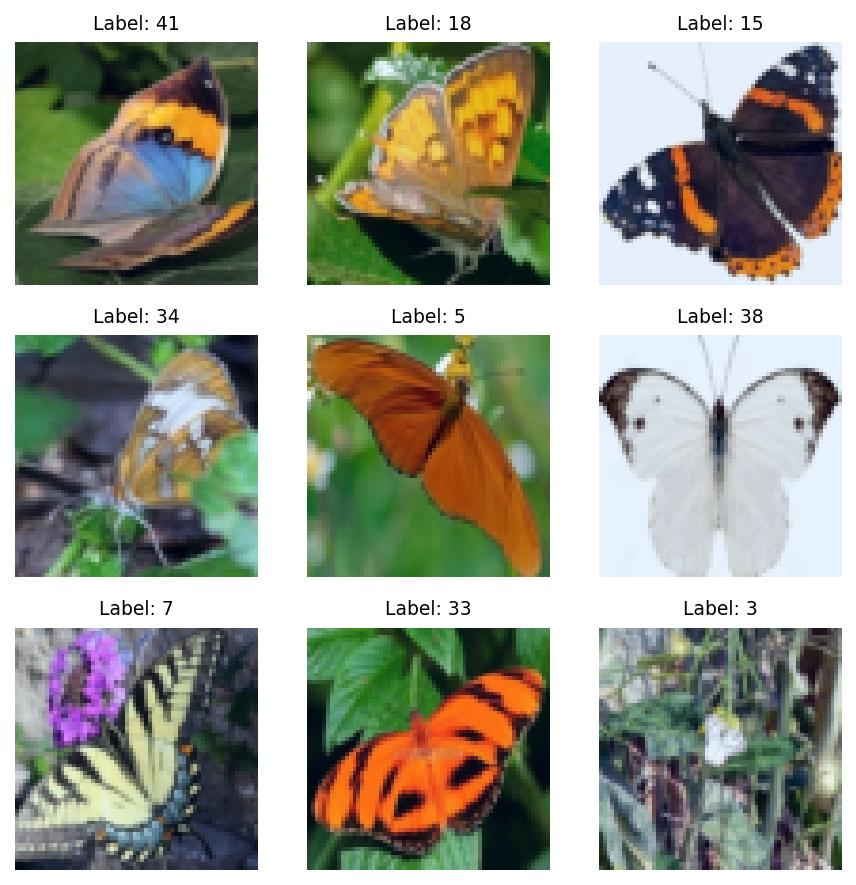
\includegraphics[width=\columnwidth]{../../images/butterfly_1_sample.jpg}
    \caption{Sample images for the Butterfly dataset.}
    \label{fig:butterfly}
\end{figure}

\subsection{Cards} This is a playing card classification dataset by rank and suit \citep{card_data}. This dataset is hosted on Kaggle and consists of 7624 images split into 53 categories. See Figure \ref{fig:cards}.

\begin{figure}[htbp]
    \centering
    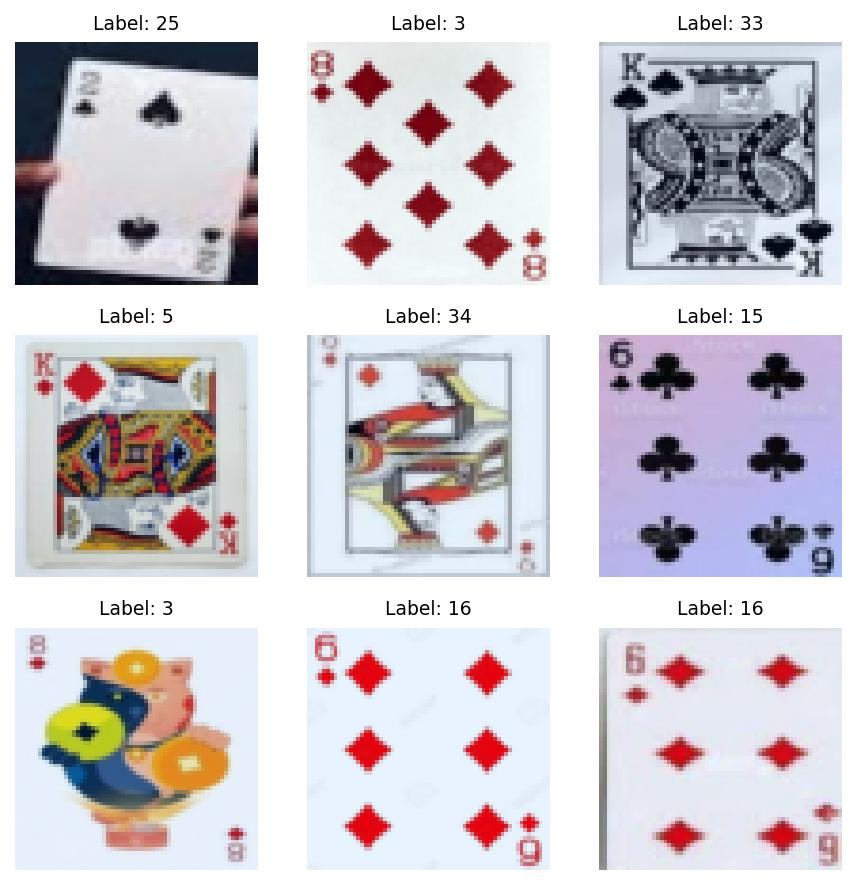
\includegraphics[width=\columnwidth]{../../images/cards_1_sample.jpg}
    \caption{Sample images for the Cards dataset.}
    \label{fig:cards}
\end{figure}


\subsection{Colon} This is a colon pathology dataset with different diseases labeled \citep{yang2023medmnist}. This dataset consists of 89,996 images in 9 different classes of colon disease. See Figure \ref{fig:colon}.


\begin{figure}[htbp]
    \centering
    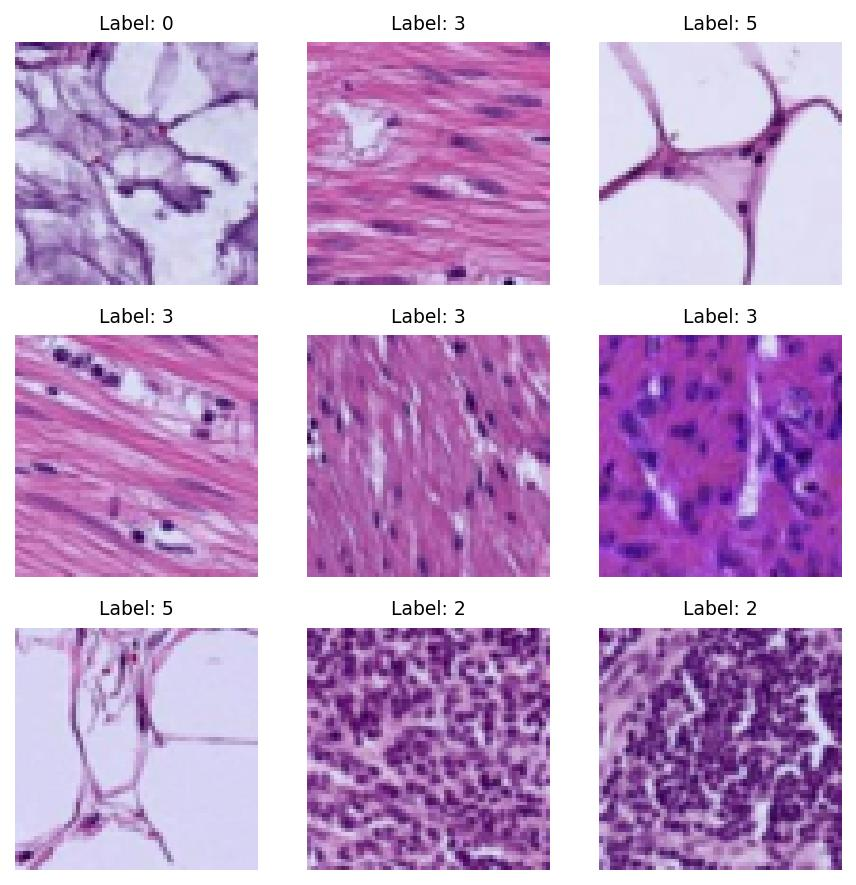
\includegraphics[width=\columnwidth]{../../images/colon_1_sample.jpg}
    \caption{Sample images for the Colon dataset.}
    \label{fig:colon}
\end{figure}

\subsection{Eurosat} This is a satellite images dataset for classifying different types of land use \citep{helber2019eurosat}. It contains 27,000 labeled images and only RGB images were used from the dataset. See Figure \ref{fig:eurosat}.

\begin{figure}[htbp]
    \centering
    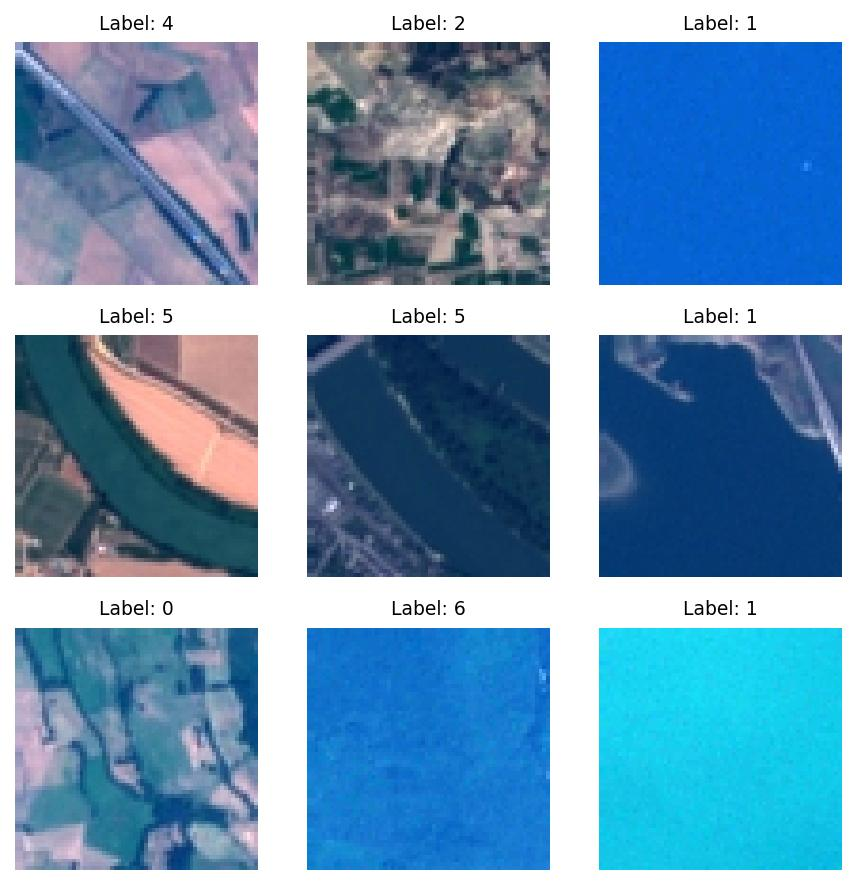
\includegraphics[width=\columnwidth]{../../images/eurosat_1_sample.jpg}
    \caption{Sample images for the Eurosat dataset.}
    \label{fig:eurosat}
\end{figure}


\subsection{Fashion} The FashionMNIST dataset describing different articles of clothing \citep{fashion}. It consists of 70,000 grey scale images labeld into 10 classes. See Figure \ref{fig:fashion}.


\begin{figure}[htbp]
    \centering
    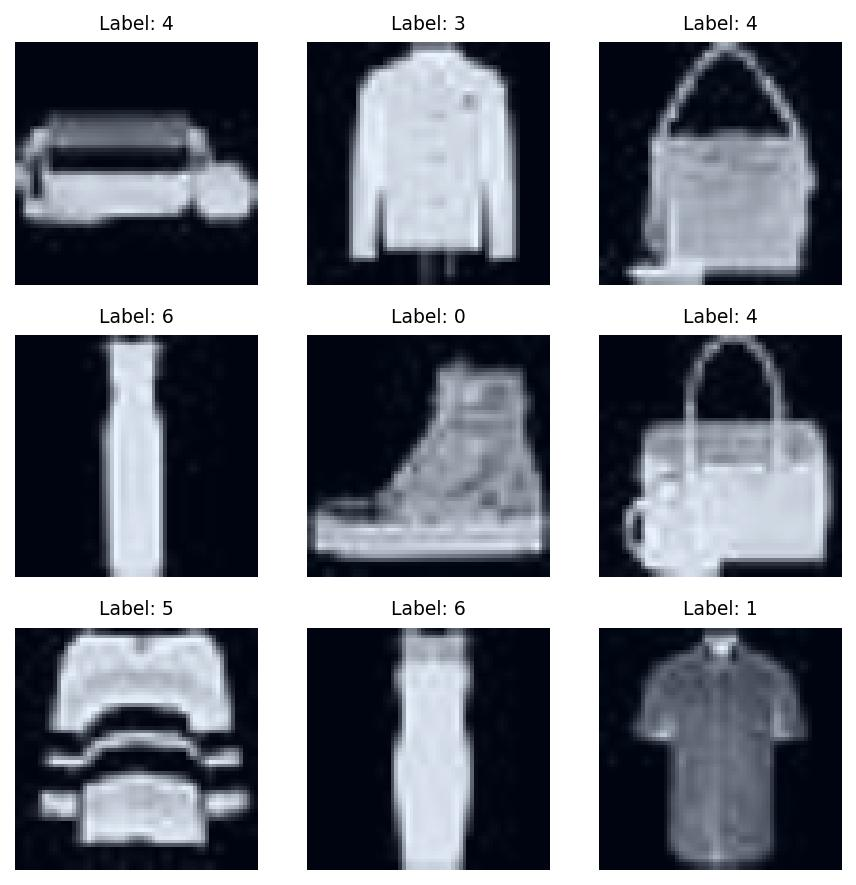
\includegraphics[width=\columnwidth]{../../images/fashion_1_sample.jpg}
    \caption{Sample images for the Fashion dataset.}
    \label{fig:fashion}
\end{figure}

\subsection{Food} The Food101 dataset \citep{food} contains $101$ classes of different types of food. It consists of 101,000 images with 1000 images per class. 

See figure \ref{fig:food}.

\begin{figure}[htbp]
    \centering
    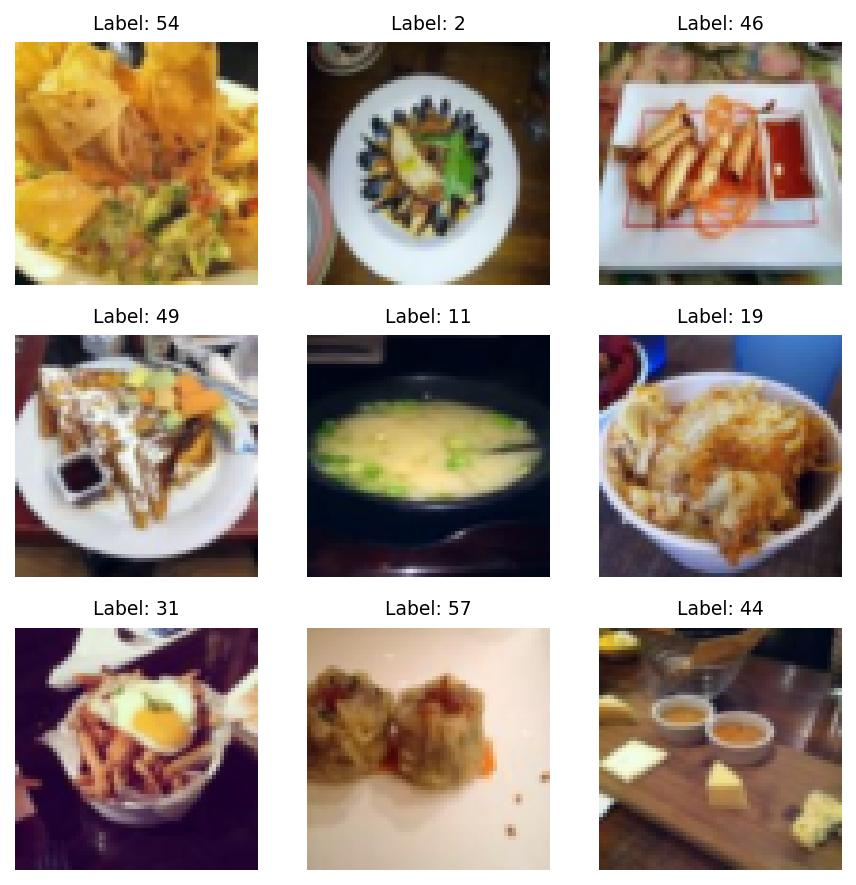
\includegraphics[width=\columnwidth]{../../images/food_1_sample.jpg}
    \caption{Sample images for the Food dataset.}
    \label{fig:food}
\end{figure}

\subsection{Garbage} This is a dataset to classify the material of different waste objects \citep{single2023realwaste}. The dataset is split into 9 classes with more than 4000 images and at least 300 images per class. See Figure \ref{fig:garbage}.

\begin{figure}[htbp]
    \centering
    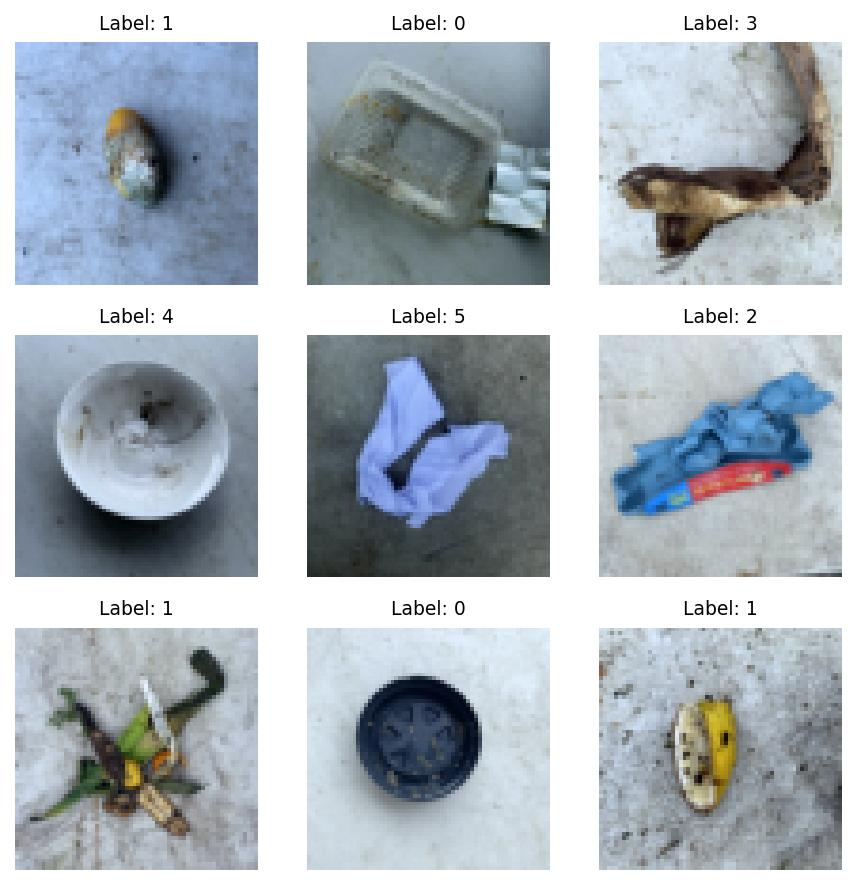
\includegraphics[width=\columnwidth]{../../images/garbage_1_sample.jpg}
    \caption{Sample images for the Garbage dataset.}
    \label{fig:garbage}
\end{figure}

\subsection{Plant} This is a plant leaves dataset detailing different types of disease \citep{plant}. There are over 50,000 images across 38 classes. Each variety of plant contains a set of healthy leaf images and one more diseased leaf images. See Figure \ref{fig:plant}.

\begin{figure}[htbp]
    \centering
    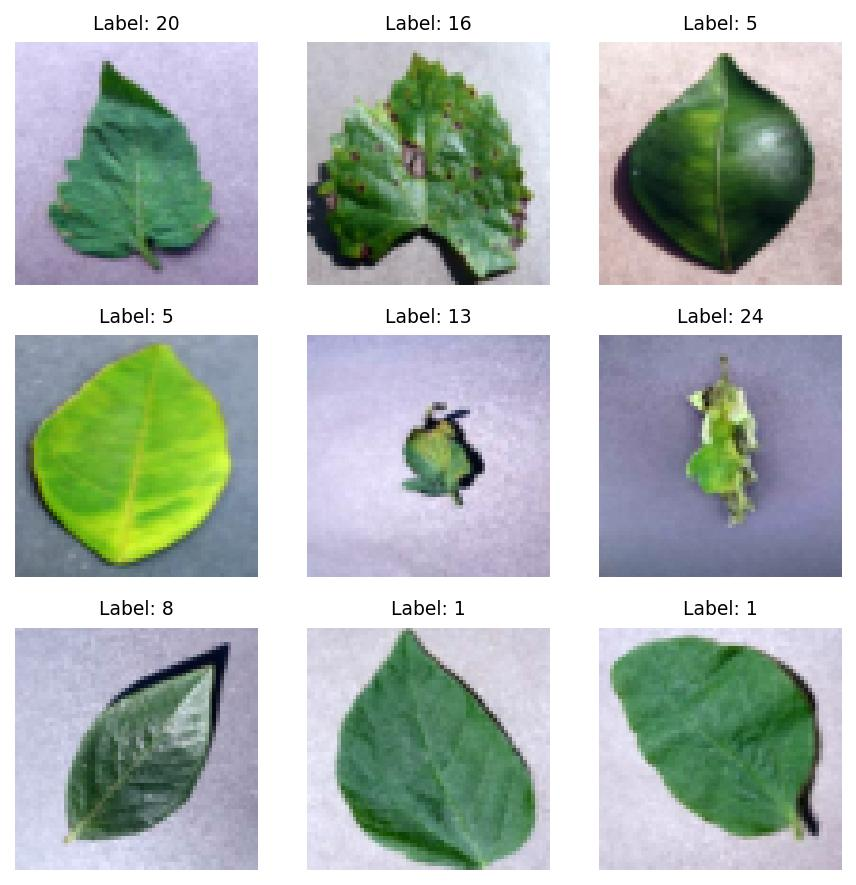
\includegraphics[width=\columnwidth]{../../images/plant_1_sample.jpg}
    \caption{Sample images for the Plant dataset.}
    \label{fig:plant}
\end{figure}

\subsection{Rock} This is a dataset of different types of rocks and minerals \citep{rock_data}. It consists of 7 different classes across more than 2000 images. See Figure \ref{fig:rock}.

\begin{figure}[htbp]
    \centering
    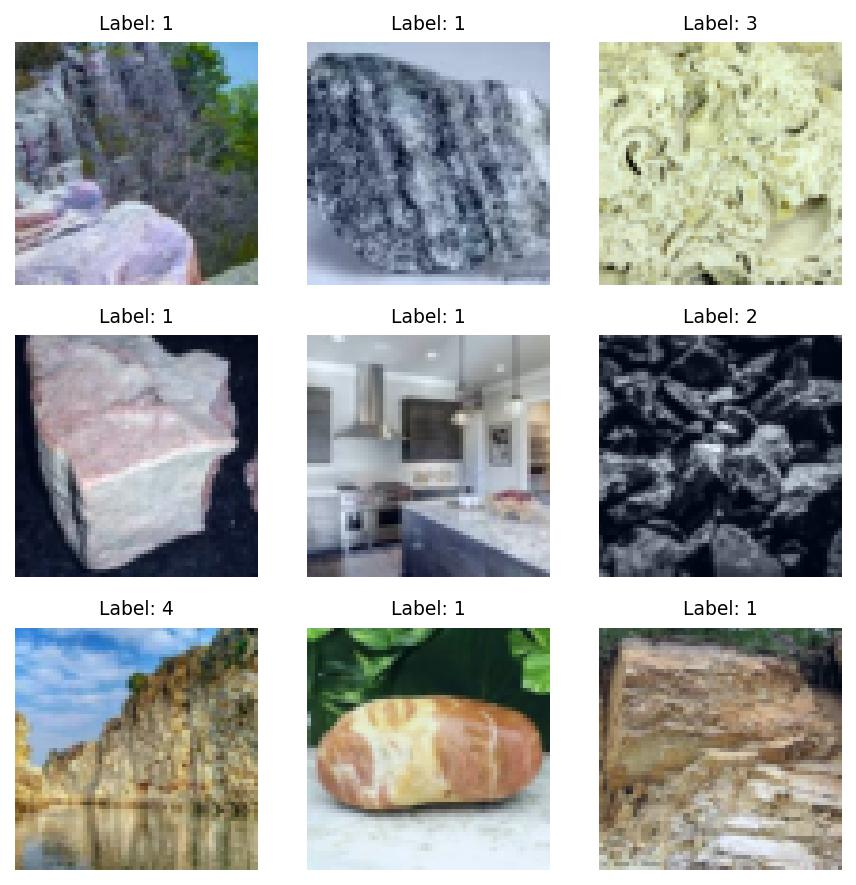
\includegraphics[width=\columnwidth]{../../images/rock_1_sample.jpg}
    \caption{Sample images for the Rock dataset. Note that this dataset appears to contain images in multiple domains, such as the kitchen image of a marble countertop.}
    \label{fig:rock}
\end{figure}



\subsection{Tissue} This is a kidney cortex microscope dataset with various types of tissue labeled \citep{yang2023medmnist}. It consists of over 200,000 images across 8 different classes. See Figure \ref{fig:tissue}

\begin{figure}[htbp]
    \centering
    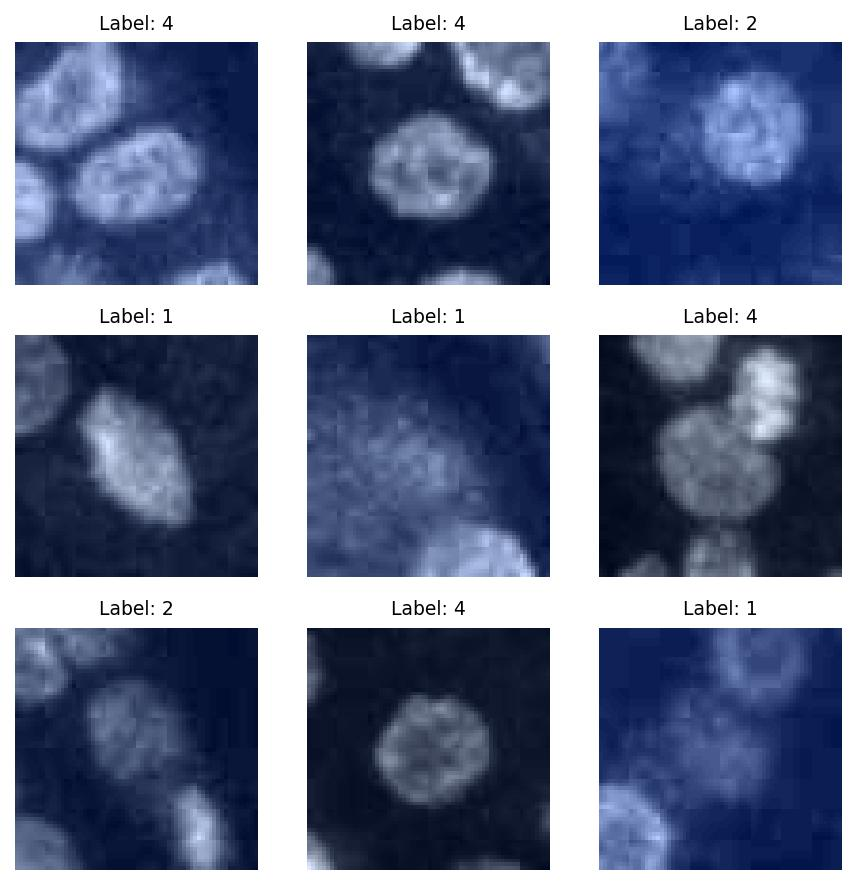
\includegraphics[width=\columnwidth]{../../images/tissue_1_sample.jpg}
    \caption{Sample images for the Tissue dataset.}
    \label{fig:tissue}
\end{figure}



\subsection{Yoga} This is a dataset of people performing different yoga poses from the internet \citep{yoga_data}. It consists of 2,964 images across 6 classes. See Figure \ref{fig:yoga}.

\begin{figure}[htbp]
    \centering
    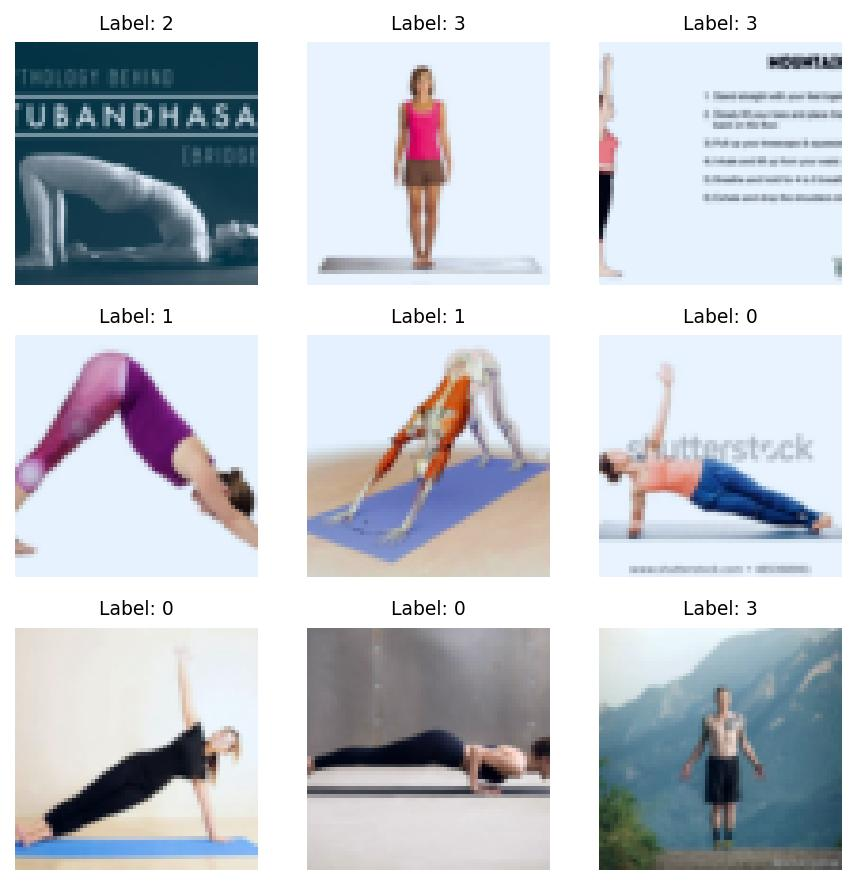
\includegraphics[width=\columnwidth]{../../images/yoga_1_sample.jpg}
    \caption{Sample images for the Yoga dataset.}
    \label{fig:yoga}
\end{figure}


\end{document}
